\documentclass[twoside]{book}

% Packages required by doxygen
\usepackage{calc}
\usepackage{doxygen}
\usepackage{graphicx}
\usepackage[utf8]{inputenc}
\usepackage{makeidx}
\usepackage{multicol}
\usepackage{multirow}
\usepackage{textcomp}
\usepackage[table]{xcolor}

% Font selection
\usepackage[T1]{fontenc}
\usepackage{mathptmx}
\usepackage[scaled=.90]{helvet}
\usepackage{courier}
\usepackage{amssymb}
\usepackage{sectsty}
\renewcommand{\familydefault}{\sfdefault}
\allsectionsfont{%
  \fontseries{bc}\selectfont%
  \color{darkgray}%
}
\renewcommand{\DoxyLabelFont}{%
  \fontseries{bc}\selectfont%
  \color{darkgray}%
}

% Page & text layout
\usepackage{geometry}
\geometry{%
  a4paper,%
  top=2.5cm,%
  bottom=2.5cm,%
  left=2.5cm,%
  right=2.5cm%
}
\tolerance=750
\hfuzz=15pt
\hbadness=750
\setlength{\emergencystretch}{15pt}
\setlength{\parindent}{0cm}
\setlength{\parskip}{0.2cm}
\makeatletter
\renewcommand{\paragraph}{%
  \@startsection{paragraph}{4}{0ex}{-1.0ex}{1.0ex}{%
    \normalfont\normalsize\bfseries\SS@parafont%
  }%
}
\renewcommand{\subparagraph}{%
  \@startsection{subparagraph}{5}{0ex}{-1.0ex}{1.0ex}{%
    \normalfont\normalsize\bfseries\SS@subparafont%
  }%
}
\makeatother

% Headers & footers
\usepackage{fancyhdr}
\pagestyle{fancyplain}
\fancyhead[LE]{\fancyplain{}{\bfseries\thepage}}
\fancyhead[CE]{\fancyplain{}{}}
\fancyhead[RE]{\fancyplain{}{\bfseries\leftmark}}
\fancyhead[LO]{\fancyplain{}{\bfseries\rightmark}}
\fancyhead[CO]{\fancyplain{}{}}
\fancyhead[RO]{\fancyplain{}{\bfseries\thepage}}
\fancyfoot[LE]{\fancyplain{}{}}
\fancyfoot[CE]{\fancyplain{}{}}
\fancyfoot[RE]{\fancyplain{}{\bfseries\scriptsize Generated on Fri Sep 20 2013 16\-:30\-:28 for Polar Plotter Project by Doxygen }}
\fancyfoot[LO]{\fancyplain{}{\bfseries\scriptsize Generated on Fri Sep 20 2013 16\-:30\-:28 for Polar Plotter Project by Doxygen }}
\fancyfoot[CO]{\fancyplain{}{}}
\fancyfoot[RO]{\fancyplain{}{}}
\renewcommand{\footrulewidth}{0.4pt}
\renewcommand{\chaptermark}[1]{%
  \markboth{#1}{}%
}
\renewcommand{\sectionmark}[1]{%
  \markright{\thesection\ #1}%
}

% Indices & bibliography
\usepackage{natbib}
\usepackage[titles]{tocloft}
\setcounter{tocdepth}{3}
\setcounter{secnumdepth}{5}
\makeindex

% Hyperlinks (required, but should be loaded last)
\usepackage{ifpdf}
\ifpdf
  \usepackage[pdftex,pagebackref=true]{hyperref}
\else
  \usepackage[ps2pdf,pagebackref=true]{hyperref}
\fi
\hypersetup{%
  colorlinks=true,%
  linkcolor=blue,%
  citecolor=blue,%
  unicode%
}

% Custom commands
\newcommand{\clearemptydoublepage}{%
  \newpage{\pagestyle{empty}\cleardoublepage}%
}


%===== C O N T E N T S =====

\begin{document}

% Titlepage & ToC
\hypersetup{pageanchor=false}
\pagenumbering{roman}
\begin{titlepage}
\vspace*{7cm}
\begin{center}%
{\Large Polar Plotter Project \\[1ex]\large 5.\-0 }\\
\vspace*{1cm}
{\large Generated by Doxygen 1.8.5}\\
\vspace*{0.5cm}
{\small Fri Sep 20 2013 16:30:28}\\
\end{center}
\end{titlepage}
\clearemptydoublepage
\tableofcontents
\clearemptydoublepage
\pagenumbering{arabic}
\hypersetup{pageanchor=true}

%--- Begin generated contents ---
\chapter{Hierarchical Index}
\section{Class Hierarchy}
This inheritance list is sorted roughly, but not completely, alphabetically\-:\begin{DoxyCompactList}
\item \contentsline{section}{da\-\_\-motor}{\pageref{classda__motor}}{}
\item \contentsline{section}{Master}{\pageref{class_master}}{}
\item \contentsline{section}{Master\-:\-:packet1}{\pageref{union_master_1_1packet1}}{}
\item \contentsline{section}{point}{\pageref{classpoint}}{}
\item \contentsline{section}{servo}{\pageref{classservo}}{}
\item stl\-\_\-task\begin{DoxyCompactList}
\item \contentsline{section}{Go\-\_\-\-Home}{\pageref{class_go___home}}{}
\item \contentsline{section}{task\-\_\-lines}{\pageref{classtask__lines}}{}
\item \contentsline{section}{task\-\_\-\-P\-I\-D}{\pageref{classtask___p_i_d}}{}
\end{DoxyCompactList}
\item \contentsline{section}{task\-\_\-print}{\pageref{classtask__print}}{}
\item \contentsline{section}{task\-\_\-read}{\pageref{classtask__read}}{}
\end{DoxyCompactList}

\chapter{Class Index}
\section{Class List}
Here are the classes, structs, unions and interfaces with brief descriptions\-:\begin{DoxyCompactList}
\item\contentsline{section}{\hyperlink{classda__motor}{da\-\_\-motor} }{\pageref{classda__motor}}{}
\item\contentsline{section}{\hyperlink{classGo__Home}{Go\-\_\-\-Home} }{\pageref{classGo__Home}}{}
\item\contentsline{section}{\hyperlink{classMaster}{Master} }{\pageref{classMaster}}{}
\item\contentsline{section}{\hyperlink{unionMaster_1_1packet1}{Master\-::packet1} \\*Encoder\-\_\-data allows easy partitioning of encoder data }{\pageref{unionMaster_1_1packet1}}{}
\item\contentsline{section}{\hyperlink{classpoint}{point} }{\pageref{classpoint}}{}
\item\contentsline{section}{\hyperlink{classservo}{servo} }{\pageref{classservo}}{}
\item\contentsline{section}{\hyperlink{classtask__lines}{task\-\_\-lines} }{\pageref{classtask__lines}}{}
\item\contentsline{section}{\hyperlink{classtask__PID}{task\-\_\-\-P\-I\-D} }{\pageref{classtask__PID}}{}
\item\contentsline{section}{\hyperlink{classtask__print}{task\-\_\-print} }{\pageref{classtask__print}}{}
\item\contentsline{section}{\hyperlink{classtask__read}{task\-\_\-read} }{\pageref{classtask__read}}{}
\end{DoxyCompactList}

\chapter{File Index}
\section{File List}
Here is a list of all documented files with brief descriptions\-:\begin{DoxyCompactList}
\item\contentsline{section}{\hyperlink{da__motor_8cpp}{da\-\_\-motor.\-cpp} }{\pageref{da__motor_8cpp}}{}
\item\contentsline{section}{\hyperlink{da__motor_8h}{da\-\_\-motor.\-h} }{\pageref{da__motor_8h}}{}
\item\contentsline{section}{\hyperlink{_go___home_8cpp}{Go\-\_\-\-Home.\-cpp} }{\pageref{_go___home_8cpp}}{}
\item\contentsline{section}{{\bfseries Go\-\_\-\-Home.\-h} }{\pageref{_go___home_8h}}{}
\item\contentsline{section}{\hyperlink{_master_8cpp}{Master.\-cpp} }{\pageref{_master_8cpp}}{}
\item\contentsline{section}{\hyperlink{_master_8h}{Master.\-h} }{\pageref{_master_8h}}{}
\item\contentsline{section}{\hyperlink{point_8cpp}{point.\-cpp} }{\pageref{point_8cpp}}{}
\item\contentsline{section}{{\bfseries point.\-h} }{\pageref{point_8h}}{}
\item\contentsline{section}{{\bfseries servo.\-h} }{\pageref{servo_8h}}{}
\item\contentsline{section}{\hyperlink{task__lines_8cpp}{task\-\_\-lines.\-cpp} }{\pageref{task__lines_8cpp}}{}
\item\contentsline{section}{\hyperlink{task__lines_8h}{task\-\_\-lines.\-h} }{\pageref{task__lines_8h}}{}
\item\contentsline{section}{\hyperlink{task___p_i_d_8cpp}{task\-\_\-\-P\-I\-D.\-cpp} }{\pageref{task___p_i_d_8cpp}}{}
\item\contentsline{section}{\hyperlink{task___p_i_d_8h}{task\-\_\-\-P\-I\-D.\-h} }{\pageref{task___p_i_d_8h}}{}
\item\contentsline{section}{{\bfseries task\-\_\-print.\-h} }{\pageref{task__print_8h}}{}
\item\contentsline{section}{{\bfseries task\-\_\-read.\-h} }{\pageref{task__read_8h}}{}
\end{DoxyCompactList}

\chapter{Class Documentation}
\hypertarget{classda__motor}{\section{da\-\_\-motor Class Reference}
\label{classda__motor}\index{da\-\_\-motor@{da\-\_\-motor}}
}


{\ttfamily \#include $<$da\-\_\-motor.\-h$>$}

\subsection*{Public Member Functions}
\begin{DoxyCompactItemize}
\item 
\hyperlink{classda__motor_acba4d745274fff811dd6bdfd2ce2e311}{da\-\_\-motor} (base\-\_\-text\-\_\-serial $\ast$)
\item 
void \hyperlink{classda__motor_ae12199588a759b98121382bfa65470cb}{set\-\_\-mode} (uint8\-\_\-t, uint8\-\_\-t)
\item 
void \hyperlink{classda__motor_aaf09074463c510eccc78f22f7df9420e}{increase\-\_\-duty\-\_\-cycle} (uint8\-\_\-t, uint8\-\_\-t $\ast$)
\item 
void \hyperlink{classda__motor_ac721f9ffd52d2ac163709eb4959ddaff}{decrease\-\_\-duty\-\_\-cycle} (uint8\-\_\-t, uint8\-\_\-t $\ast$)
\item 
void \hyperlink{classda__motor_a4327ab2965cece1442288893ec880e0c}{update\-\_\-duty\-\_\-cycle} (uint8\-\_\-t, uint8\-\_\-t)
\end{DoxyCompactItemize}
\subsection*{Protected Attributes}
\begin{DoxyCompactItemize}
\item 
\hypertarget{classda__motor_a31d8bcb129ad32f429176f4c04e8a572}{base\-\_\-text\-\_\-serial $\ast$ {\bfseries ptr\-\_\-to\-\_\-serial}}\label{classda__motor_a31d8bcb129ad32f429176f4c04e8a572}

\end{DoxyCompactItemize}


\subsection{Detailed Description}
\hyperlink{da__motor_8cpp}{da\-\_\-motor.\-cpp} is an object class that contains a constructor and three methods which control a motor(s). The constructor initializes timers, prescalars and configures necessary i/o ports. Two of the three methods are mirror images of each other and are used to increase/decrease rotational speed. The final method sets the H bridge to achieve proper rotational direction and braking. 

Definition at line 26 of file da\-\_\-motor.\-h.



\subsection{Constructor \& Destructor Documentation}
\hypertarget{classda__motor_acba4d745274fff811dd6bdfd2ce2e311}{\index{da\-\_\-motor@{da\-\_\-motor}!da\-\_\-motor@{da\-\_\-motor}}
\index{da\-\_\-motor@{da\-\_\-motor}!da_motor@{da\-\_\-motor}}
\subsubsection[{da\-\_\-motor}]{\setlength{\rightskip}{0pt plus 5cm}da\-\_\-motor\-::da\-\_\-motor (
\begin{DoxyParamCaption}
\item[{base\-\_\-text\-\_\-serial $\ast$}]{p\-\_\-serial\-\_\-port}
\end{DoxyParamCaption}
)}}\label{classda__motor_acba4d745274fff811dd6bdfd2ce2e311}
This constructor configures the P\-W\-M timer on the A\-Tmega128 and the H-\/bridges on the V\-N\-H motor driver chips set up a motor driver. 
\begin{DoxyParams}{Parameters}
{\em p\-\_\-serial\-\_\-port} & A pointer to the serial port which writes debugging info. \\
\hline
\end{DoxyParams}


Definition at line 22 of file da\-\_\-motor.\-cpp.



\subsection{Member Function Documentation}
\hypertarget{classda__motor_ac721f9ffd52d2ac163709eb4959ddaff}{\index{da\-\_\-motor@{da\-\_\-motor}!decrease\-\_\-duty\-\_\-cycle@{decrease\-\_\-duty\-\_\-cycle}}
\index{decrease\-\_\-duty\-\_\-cycle@{decrease\-\_\-duty\-\_\-cycle}!da_motor@{da\-\_\-motor}}
\subsubsection[{decrease\-\_\-duty\-\_\-cycle}]{\setlength{\rightskip}{0pt plus 5cm}void da\-\_\-motor\-::decrease\-\_\-duty\-\_\-cycle (
\begin{DoxyParamCaption}
\item[{uint8\-\_\-t}]{motor\-\_\-num, }
\item[{uint8\-\_\-t $\ast$}]{duty\-\_\-cycle}
\end{DoxyParamCaption}
)}}\label{classda__motor_ac721f9ffd52d2ac163709eb4959ddaff}
manually decrease the duty cycle by 2\% \hyperlink{classda__motor_ac721f9ffd52d2ac163709eb4959ddaff}{da\-\_\-motor.\-decrease\-\_\-duty\-\_\-cycle} allows a user to decrease the rotational speed of a motor. The motor who's speed is adjusted is whichever motor (1 or 2) was previously selected. 
\begin{DoxyParams}{Parameters}
{\em motor\-\_\-num,\-:} & determines which motor is adjusted \\
\hline
{\em duty\-\_\-cycle,\-:} & a pointer to duty\-\_\-cycle allows this method to alter values in duty cycle (a variable in main) \\
\hline
\end{DoxyParams}


Definition at line 164 of file da\-\_\-motor.\-cpp.

\hypertarget{classda__motor_aaf09074463c510eccc78f22f7df9420e}{\index{da\-\_\-motor@{da\-\_\-motor}!increase\-\_\-duty\-\_\-cycle@{increase\-\_\-duty\-\_\-cycle}}
\index{increase\-\_\-duty\-\_\-cycle@{increase\-\_\-duty\-\_\-cycle}!da_motor@{da\-\_\-motor}}
\subsubsection[{increase\-\_\-duty\-\_\-cycle}]{\setlength{\rightskip}{0pt plus 5cm}void da\-\_\-motor\-::increase\-\_\-duty\-\_\-cycle (
\begin{DoxyParamCaption}
\item[{uint8\-\_\-t}]{motor\-\_\-num, }
\item[{uint8\-\_\-t $\ast$}]{duty\-\_\-cycle}
\end{DoxyParamCaption}
)}}\label{classda__motor_aaf09074463c510eccc78f22f7df9420e}
manually increase the duty cycle by 2\% \hyperlink{classda__motor_aaf09074463c510eccc78f22f7df9420e}{da\-\_\-motor.\-increase\-\_\-duty\-\_\-cycle} allows a user to increase the rotational speed of a motor. The motor who's speed is adjusted is whichever motor (1 or 2) was previously selected. 
\begin{DoxyParams}{Parameters}
{\em motor\-\_\-num,\-:} & determines which motor is adjusted \\
\hline
{\em duty\-\_\-cycle,\-:} & a pointer to duty\-\_\-cycle allows this method to alter values in duty cycle (a variable in main) \\
\hline
\end{DoxyParams}


Definition at line 131 of file da\-\_\-motor.\-cpp.

\hypertarget{classda__motor_ae12199588a759b98121382bfa65470cb}{\index{da\-\_\-motor@{da\-\_\-motor}!set\-\_\-mode@{set\-\_\-mode}}
\index{set\-\_\-mode@{set\-\_\-mode}!da_motor@{da\-\_\-motor}}
\subsubsection[{set\-\_\-mode}]{\setlength{\rightskip}{0pt plus 5cm}void da\-\_\-motor\-::set\-\_\-mode (
\begin{DoxyParamCaption}
\item[{uint8\-\_\-t}]{motor\-\_\-num, }
\item[{uint8\-\_\-t}]{mode}
\end{DoxyParamCaption}
)}}\label{classda__motor_ae12199588a759b98121382bfa65470cb}
\hyperlink{classda__motor_ae12199588a759b98121382bfa65470cb}{da\-\_\-motor.\-set\-\_\-mode} allows a user to choose a motor's rotational direction or apply unmodulated braking. These tasks are performed by passing motor\-\_\-num a 1 or a 2 to select which motor's state to change and mode a 1, 2, or 3. 
\begin{DoxyParams}{Parameters}
{\em motor\-\_\-num,\-:} & selects motor number 1 or 2. \\
\hline
{\em mode,\-:} & mode 1 = spin C\-W mode 2 = spin C\-C\-W mode 3 = unmodulated braking. \\
\hline
\end{DoxyParams}


Definition at line 76 of file da\-\_\-motor.\-cpp.



Referenced by Go\-\_\-\-Home\-::run(), and task\-\_\-\-P\-I\-D\-::run().

\hypertarget{classda__motor_a4327ab2965cece1442288893ec880e0c}{\index{da\-\_\-motor@{da\-\_\-motor}!update\-\_\-duty\-\_\-cycle@{update\-\_\-duty\-\_\-cycle}}
\index{update\-\_\-duty\-\_\-cycle@{update\-\_\-duty\-\_\-cycle}!da_motor@{da\-\_\-motor}}
\subsubsection[{update\-\_\-duty\-\_\-cycle}]{\setlength{\rightskip}{0pt plus 5cm}void da\-\_\-motor\-::update\-\_\-duty\-\_\-cycle (
\begin{DoxyParamCaption}
\item[{uint8\-\_\-t}]{motor\-\_\-num, }
\item[{uint8\-\_\-t}]{duty\-\_\-cycle}
\end{DoxyParamCaption}
)}}\label{classda__motor_a4327ab2965cece1442288893ec880e0c}
update\-\_\-duty\-\_\-cycle is a method which allows you to update the a motor's duty cycle with any 8-\/bit value you want instead of incrementally. 

Definition at line 191 of file da\-\_\-motor.\-cpp.



Referenced by Go\-\_\-\-Home\-::run(), and task\-\_\-\-P\-I\-D\-::run().



The documentation for this class was generated from the following files\-:\begin{DoxyCompactItemize}
\item 
\hyperlink{da__motor_8h}{da\-\_\-motor.\-h}\item 
\hyperlink{da__motor_8cpp}{da\-\_\-motor.\-cpp}\end{DoxyCompactItemize}

\hypertarget{classGo__Home}{\section{Go\-\_\-\-Home Class Reference}
\label{classGo__Home}\index{Go\-\_\-\-Home@{Go\-\_\-\-Home}}
}


{\ttfamily \#include $<$Go\-\_\-\-Home.\-h$>$}

Inheritance diagram for Go\-\_\-\-Home\-:\begin{figure}[H]
\begin{center}
\leavevmode
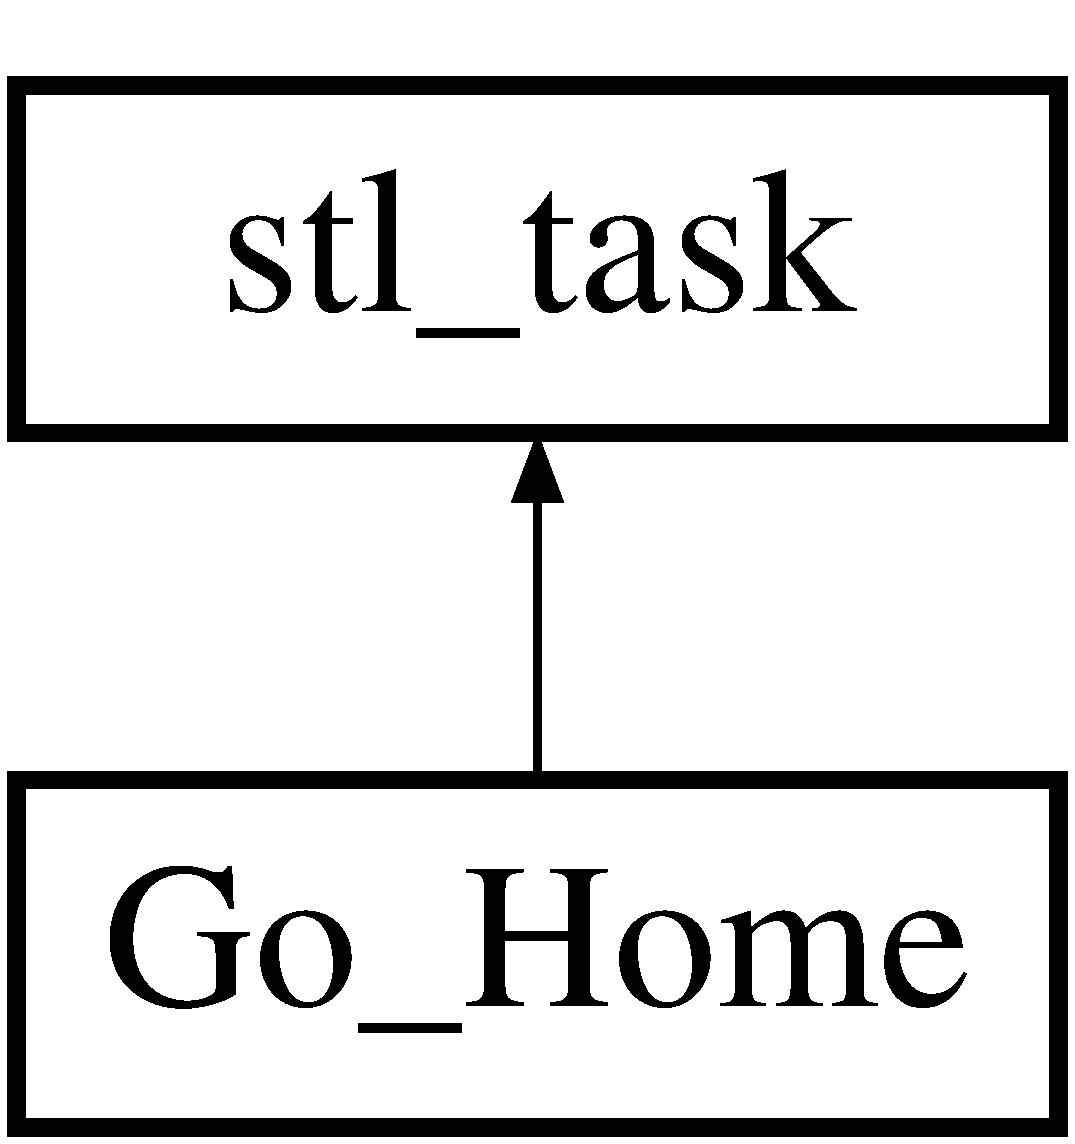
\includegraphics[height=2.000000cm]{classGo__Home}
\end{center}
\end{figure}
\subsection*{Public Member Functions}
\begin{DoxyCompactItemize}
\item 
\hyperlink{classGo__Home_a080085bcc6207561d5309d5f861b10cf}{Go\-\_\-\-Home} (base\-\_\-text\-\_\-serial $\ast$, task\-\_\-timer \&, time\-\_\-stamp \&, \hyperlink{classda__motor}{da\-\_\-motor} $\ast$, \hyperlink{classMaster}{Master} $\ast$, \hyperlink{classtask__PID}{task\-\_\-\-P\-I\-D} $\ast$, \hyperlink{classtask__PID}{task\-\_\-\-P\-I\-D} $\ast$, \hyperlink{classtask__lines}{task\-\_\-lines} $\ast$)
\item 
char \hyperlink{classGo__Home_ae1421efd3ca49627022675f74534ced6}{run} (char state)
\item 
void \hyperlink{classGo__Home_a1c22463a7cca8fd6a8ab4c5c9ecee6ff}{S\-E\-T\-\_\-\-Home\-\_\-\-Request} (void)
\item 
bool \hyperlink{classGo__Home_a23ee51618c74f918af0ddf4555c7ff04}{Is\-\_\-\-Home} (void)
\end{DoxyCompactItemize}
\subsection*{Protected Attributes}
\begin{DoxyCompactItemize}
\item 
\hypertarget{classGo__Home_aaf0a0c125f002315ced04f6a2520faff}{base\-\_\-text\-\_\-serial $\ast$ {\bfseries ptr\-\_\-2\-\_\-serial}}\label{classGo__Home_aaf0a0c125f002315ced04f6a2520faff}

\item 
\hypertarget{classGo__Home_a27906c7ed2cef0678fe85e7024252795}{\hyperlink{classda__motor}{da\-\_\-motor} $\ast$ {\bfseries Vtec\-\_\-wins}}\label{classGo__Home_a27906c7ed2cef0678fe85e7024252795}

\item 
\hypertarget{classGo__Home_a43872cca289815689ac830135c3d58f1}{\hyperlink{classMaster}{Master} $\ast$ {\bfseries Wipe\-\_\-\-Slave}}\label{classGo__Home_a43872cca289815689ac830135c3d58f1}

\item 
\hypertarget{classGo__Home_a57ef328cc70eabbb8668c048aad96a8d}{\hyperlink{classtask__PID}{task\-\_\-\-P\-I\-D} $\ast$ {\bfseries Wipe\-\_\-\-Master1}}\label{classGo__Home_a57ef328cc70eabbb8668c048aad96a8d}

\item 
\hypertarget{classGo__Home_adf786b11550fc9149035ed7edc398133}{\hyperlink{classtask__PID}{task\-\_\-\-P\-I\-D} $\ast$ {\bfseries Wipe\-\_\-\-Master2}}\label{classGo__Home_adf786b11550fc9149035ed7edc398133}

\item 
\hypertarget{classGo__Home_a5e9d6df4b4ee935e5266487bc9ce2fda}{\hyperlink{classtask__lines}{task\-\_\-lines} $\ast$ {\bfseries L\-I\-N\-E\-S}}\label{classGo__Home_a5e9d6df4b4ee935e5266487bc9ce2fda}

\end{DoxyCompactItemize}


\subsection{Detailed Description}
\hyperlink{Go__Home_8cpp}{Go\-\_\-\-Home.\-cpp} is a class with methods to send the carriage and arm to their home positions and reset both motor encoders. Two bump-\/stop switches connected to pin interrupts tell the microcontroller to stop the motors when the carriage and arm reach their respective home positions. 

Definition at line 23 of file Go\-\_\-\-Home.\-h.



\subsection{Constructor \& Destructor Documentation}
\hypertarget{classGo__Home_a080085bcc6207561d5309d5f861b10cf}{\index{Go\-\_\-\-Home@{Go\-\_\-\-Home}!Go\-\_\-\-Home@{Go\-\_\-\-Home}}
\index{Go\-\_\-\-Home@{Go\-\_\-\-Home}!Go_Home@{Go\-\_\-\-Home}}
\subsubsection[{Go\-\_\-\-Home}]{\setlength{\rightskip}{0pt plus 5cm}Go\-\_\-\-Home\-::\-Go\-\_\-\-Home (
\begin{DoxyParamCaption}
\item[{base\-\_\-text\-\_\-serial $\ast$}]{p\-\_\-serial\-\_\-port, }
\item[{task\-\_\-timer \&}]{a\-\_\-timer, }
\item[{time\-\_\-stamp \&}]{t\-\_\-stamp, }
\item[{{\bf da\-\_\-motor} $\ast$}]{Vortec, }
\item[{{\bf Master} $\ast$}]{Clear\-\_\-\-Slave, }
\item[{{\bf task\-\_\-\-P\-I\-D} $\ast$}]{Clear\-\_\-\-Master1, }
\item[{{\bf task\-\_\-\-P\-I\-D} $\ast$}]{Clear\-\_\-\-Master2, }
\item[{{\bf task\-\_\-lines} $\ast$}]{liner}
\end{DoxyParamCaption}
)}}\label{classGo__Home_a080085bcc6207561d5309d5f861b10cf}
This constructor enables the interrupts necessary for the bump stop switches on our plotter to operate, initializes control booleans, and saves object pointers locally. 
\begin{DoxyParams}{Parameters}
{\em p\-\_\-serial\-\_\-port} & Allows screen printouts \\
\hline
{\em a\-\_\-timer,\-:} & A Timer object to assist with sceduling \\
\hline
{\em t\-\_\-stamp,\-:} & A Time Stamp object to assist with sceduling \\
\hline
{\em Vortec,\-:} & A motor object \\
\hline
{\em Clear\-\_\-\-Slave} & An S\-P\-I master object \\
\hline
{\em Clear\-\_\-\-Master1} & P\-I\-D object for motor 1 \\
\hline
{\em Clear\-\_\-\-Master2} & P\-I\-D object for motor 2 \\
\hline
{\em liner} & task lines object so it can call home \\
\hline
\end{DoxyParams}


Definition at line 44 of file Go\-\_\-\-Home.\-cpp.



\subsection{Member Function Documentation}
\hypertarget{classGo__Home_a23ee51618c74f918af0ddf4555c7ff04}{\index{Go\-\_\-\-Home@{Go\-\_\-\-Home}!Is\-\_\-\-Home@{Is\-\_\-\-Home}}
\index{Is\-\_\-\-Home@{Is\-\_\-\-Home}!Go_Home@{Go\-\_\-\-Home}}
\subsubsection[{Is\-\_\-\-Home}]{\setlength{\rightskip}{0pt plus 5cm}bool Go\-\_\-\-Home\-::\-Is\-\_\-\-Home (
\begin{DoxyParamCaption}
\item[{void}]{}
\end{DoxyParamCaption}
)}}\label{classGo__Home_a23ee51618c74f918af0ddf4555c7ff04}
Is\-\_\-\-Home returns a flag which is true if machine is done homing. 

Definition at line 154 of file Go\-\_\-\-Home.\-cpp.



References Home\-\_\-\-Request.

\hypertarget{classGo__Home_ae1421efd3ca49627022675f74534ced6}{\index{Go\-\_\-\-Home@{Go\-\_\-\-Home}!run@{run}}
\index{run@{run}!Go_Home@{Go\-\_\-\-Home}}
\subsubsection[{run}]{\setlength{\rightskip}{0pt plus 5cm}char Go\-\_\-\-Home\-::run (
\begin{DoxyParamCaption}
\item[{char}]{state}
\end{DoxyParamCaption}
)}}\label{classGo__Home_ae1421efd3ca49627022675f74534ced6}
run is the main method in \hyperlink{classGo__Home}{Go\-\_\-\-Home} and it performs the actual homing operation of the 2 degree of freedom system. 
\begin{DoxyParams}{Parameters}
{\em state,\-:} & S\-T\-L\-\_\-task is used for scheduling \\
\hline
\end{DoxyParams}
State 0 does nothing unless homing is requested by user key press or \hyperlink{classtask__lines}{task\-\_\-lines}

State 1 initiates movement of the arm towards home if cart has reached r=0

State 2 concludes homing once arm reaches T\-H\-E\-T\-A=0. 

Definition at line 71 of file Go\-\_\-\-Home.\-cpp.



References arm\-\_\-switch, cart\-\_\-switch, Master\-::\-C\-L\-E\-A\-R(), task\-\_\-\-P\-I\-D\-::\-C\-L\-E\-A\-R(), Home\-\_\-\-Request, task\-\_\-lines\-::ok\-\_\-were\-\_\-home(), task\-\_\-\-P\-I\-D\-::\-Request\-\_\-\-Home(), da\-\_\-motor\-::set\-\_\-mode(), da\-\_\-motor\-::update\-\_\-duty\-\_\-cycle(), and task\-\_\-lines\-::wanna\-\_\-go\-\_\-home().

\hypertarget{classGo__Home_a1c22463a7cca8fd6a8ab4c5c9ecee6ff}{\index{Go\-\_\-\-Home@{Go\-\_\-\-Home}!S\-E\-T\-\_\-\-Home\-\_\-\-Request@{S\-E\-T\-\_\-\-Home\-\_\-\-Request}}
\index{S\-E\-T\-\_\-\-Home\-\_\-\-Request@{S\-E\-T\-\_\-\-Home\-\_\-\-Request}!Go_Home@{Go\-\_\-\-Home}}
\subsubsection[{S\-E\-T\-\_\-\-Home\-\_\-\-Request}]{\setlength{\rightskip}{0pt plus 5cm}void Go\-\_\-\-Home\-::\-S\-E\-T\-\_\-\-Home\-\_\-\-Request (
\begin{DoxyParamCaption}
\item[{void}]{}
\end{DoxyParamCaption}
)}}\label{classGo__Home_a1c22463a7cca8fd6a8ab4c5c9ecee6ff}
S\-E\-T\-\_\-\-Home\-\_\-\-Request allows homing to be initiated by other tasks 

Definition at line 147 of file Go\-\_\-\-Home.\-cpp.



References Home\-\_\-\-Request.



Referenced by task\-\_\-read\-::run().



The documentation for this class was generated from the following files\-:\begin{DoxyCompactItemize}
\item 
Go\-\_\-\-Home.\-h\item 
\hyperlink{Go__Home_8cpp}{Go\-\_\-\-Home.\-cpp}\end{DoxyCompactItemize}

\hypertarget{classMaster}{\section{Master Class Reference}
\label{classMaster}\index{Master@{Master}}
}


{\ttfamily \#include $<$Master.\-h$>$}

\subsection*{Classes}
\begin{DoxyCompactItemize}
\item 
union \hyperlink{unionMaster_1_1packet1}{packet1}
\begin{DoxyCompactList}\small\item\em encoder\-\_\-data allows easy partitioning of encoder data \end{DoxyCompactList}\end{DoxyCompactItemize}
\subsection*{Public Member Functions}
\begin{DoxyCompactItemize}
\item 
\hyperlink{classMaster_a39589d526331f8b5abf9d405a5ea7fe7}{Master} (base\-\_\-text\-\_\-serial $\ast$)
\item 
void \hyperlink{classMaster_ad85c13cad19e5600c6d2dff28aaa0a52}{C\-L\-E\-A\-R} (uint8\-\_\-t)
\item 
void \hyperlink{classMaster_af507aba60a24105be4b58a441780fa28}{Initiate} (uint8\-\_\-t)
\item 
bool \hyperlink{classMaster_af5baf3043c5c903472a906cd29643725}{Get\-\_\-\-Checksum\-\_\-flag} (void)
\item 
uint8\-\_\-t \hyperlink{classMaster_ac93f188774888e736f1bcb3345e6f208}{Get\-\_\-\-Checksum\-\_\-\-Error} (void)
\item 
int32\-\_\-t \hyperlink{classMaster_ac6036259c4c2c8f4f3a11fd36ae23a6b}{Get\-\_\-\-Encoder} (void)
\end{DoxyCompactItemize}
\subsection*{Protected Attributes}
\begin{DoxyCompactItemize}
\item 
\hypertarget{classMaster_a826ae7a92e5910b4bf275a128a5aafc0}{base\-\_\-text\-\_\-serial $\ast$ \hyperlink{classMaster_a826ae7a92e5910b4bf275a128a5aafc0}{ptr\-\_\-to\-\_\-serial}}\label{classMaster_a826ae7a92e5910b4bf275a128a5aafc0}

\begin{DoxyCompactList}\small\item\em The encoder driver class needs a pointer to the serial port used to output to the terminal. \end{DoxyCompactList}\item 
\hypertarget{classMaster_a4c51d672c465103b0e3a85ff5ae68d79}{bool \hyperlink{classMaster_a4c51d672c465103b0e3a85ff5ae68d79}{error\-\_\-flag}}\label{classMaster_a4c51d672c465103b0e3a85ff5ae68d79}

\begin{DoxyCompactList}\small\item\em flag indicating transfer error on encoder 1 \end{DoxyCompactList}\item 
\hypertarget{classMaster_a3183754384c4bfd6a920c82e5e3b1618}{int32\-\_\-t \hyperlink{classMaster_a3183754384c4bfd6a920c82e5e3b1618}{encoder}}\label{classMaster_a3183754384c4bfd6a920c82e5e3b1618}

\begin{DoxyCompactList}\small\item\em encoder value received from Slave\-\_\-\-Driver \end{DoxyCompactList}\item 
\hypertarget{classMaster_a65e5841164cc7b6e5c5501c12e5a797a}{uint8\-\_\-t \hyperlink{classMaster_a65e5841164cc7b6e5c5501c12e5a797a}{Checksum\-\_\-\-Error}}\label{classMaster_a65e5841164cc7b6e5c5501c12e5a797a}

\begin{DoxyCompactList}\small\item\em encoder transfer error 1 \end{DoxyCompactList}\item 
\hypertarget{classMaster_a1d30123857f1025903e8b6d8a30cff95}{uint8\-\_\-t \hyperlink{classMaster_a1d30123857f1025903e8b6d8a30cff95}{Check\-\_\-\-Sum\-\_\-\-Master}}\label{classMaster_a1d30123857f1025903e8b6d8a30cff95}

\begin{DoxyCompactList}\small\item\em check sum computed here in master for encoder 1 \end{DoxyCompactList}\item 
\hypertarget{classMaster_a7231699fbe88393c0d0ff693253f983a}{uint8\-\_\-t \hyperlink{classMaster_a7231699fbe88393c0d0ff693253f983a}{Slave\-\_\-\-Sum}}\label{classMaster_a7231699fbe88393c0d0ff693253f983a}

\begin{DoxyCompactList}\small\item\em check sum computed in slave for encoder 1 \end{DoxyCompactList}\item 
\hypertarget{classMaster_a113205aa4218d33663faeeede6b1e8a9}{uint8\-\_\-t \hyperlink{classMaster_a113205aa4218d33663faeeede6b1e8a9}{dummy}}\label{classMaster_a113205aa4218d33663faeeede6b1e8a9}

\begin{DoxyCompactList}\small\item\em counter used to delay so S\-P\-I works \end{DoxyCompactList}\item 
\hypertarget{classMaster_a1e3e8189d315b4bf7415fe03f4035a10}{uint8\-\_\-t \hyperlink{classMaster_a1e3e8189d315b4bf7415fe03f4035a10}{encoder\-\_\-num}}\label{classMaster_a1e3e8189d315b4bf7415fe03f4035a10}

\begin{DoxyCompactList}\small\item\em integer to tell \hyperlink{classMaster}{Master} which encoder reading to get from Slave\-\_\-\-Driver \end{DoxyCompactList}\item 
\hypertarget{classMaster_a96b723e105507a410c9d0e56398174f0}{union \hyperlink{unionMaster_1_1packet1}{Master\-::packet1} {\bfseries encoder\-\_\-data}}\label{classMaster_a96b723e105507a410c9d0e56398174f0}

\end{DoxyCompactItemize}


\subsection{Detailed Description}
\hyperlink{Master_8cpp}{Master.\-cpp} is a class with methods for orchestrating and controlling the flow of data transfers on the S\-P\-I bus between a master device and a slave device. The data being transfered are new encoder positions from the two motors so that the \hyperlink{classtask__PID}{task\-\_\-\-P\-I\-D} class can keep track of where the motors are. The encoder values used in the P\-I\-D calculations are stored in the main program and are updated in \hyperlink{classMaster}{Master} via pointers so that other objects can use them as well. 

Definition at line 31 of file Master.\-h.



\subsection{Constructor \& Destructor Documentation}
\hypertarget{classMaster_a39589d526331f8b5abf9d405a5ea7fe7}{\index{Master@{Master}!Master@{Master}}
\index{Master@{Master}!Master@{Master}}
\subsubsection[{Master}]{\setlength{\rightskip}{0pt plus 5cm}Master\-::\-Master (
\begin{DoxyParamCaption}
\item[{base\-\_\-text\-\_\-serial $\ast$}]{p\-\_\-serial\-\_\-port}
\end{DoxyParamCaption}
)}}\label{classMaster_a39589d526331f8b5abf9d405a5ea7fe7}
The constructor takes in a serial pointer and saves it locally and constructs a \hyperlink{classMaster}{Master} object. The object sets up S\-P\-I communications as a master. 
\begin{DoxyParams}{Parameters}
{\em p\-\_\-serial\-\_\-port} & serial object to allow printing \\
\hline
\end{DoxyParams}


Definition at line 25 of file Master.\-cpp.



References C\-L\-E\-A\-R(), and ptr\-\_\-to\-\_\-serial.



\subsection{Member Function Documentation}
\hypertarget{classMaster_ad85c13cad19e5600c6d2dff28aaa0a52}{\index{Master@{Master}!C\-L\-E\-A\-R@{C\-L\-E\-A\-R}}
\index{C\-L\-E\-A\-R@{C\-L\-E\-A\-R}!Master@{Master}}
\subsubsection[{C\-L\-E\-A\-R}]{\setlength{\rightskip}{0pt plus 5cm}void Master\-::\-C\-L\-E\-A\-R (
\begin{DoxyParamCaption}
\item[{uint8\-\_\-t}]{motor\-\_\-num}
\end{DoxyParamCaption}
)}}\label{classMaster_ad85c13cad19e5600c6d2dff28aaa0a52}
Clear is a method to clear a pair of counters located on another chip. Associated values in this class are also cleared 
\begin{DoxyParams}{Parameters}
{\em motor\-\_\-num} & pass in the value of which motor's encoder you would like to reset. motor\-\_\-num=1 corresponds to command 3 and motor\-\_\-num=2 sends command 4. \\
\hline
\end{DoxyParams}


Definition at line 53 of file Master.\-cpp.



References Checksum\-\_\-\-Error, dummy, encoder, and ptr\-\_\-to\-\_\-serial.



Referenced by Master(), and Go\-\_\-\-Home\-::run().

\hypertarget{classMaster_ac93f188774888e736f1bcb3345e6f208}{\index{Master@{Master}!Get\-\_\-\-Checksum\-\_\-\-Error@{Get\-\_\-\-Checksum\-\_\-\-Error}}
\index{Get\-\_\-\-Checksum\-\_\-\-Error@{Get\-\_\-\-Checksum\-\_\-\-Error}!Master@{Master}}
\subsubsection[{Get\-\_\-\-Checksum\-\_\-\-Error}]{\setlength{\rightskip}{0pt plus 5cm}uint8\-\_\-t Master\-::\-Get\-\_\-\-Checksum\-\_\-\-Error (
\begin{DoxyParamCaption}
\item[{void}]{}
\end{DoxyParamCaption}
)}}\label{classMaster_ac93f188774888e736f1bcb3345e6f208}
Get\-\_\-\-Checksum\-\_\-\-Error gets the number of encoder transfer errors experienced 

Definition at line 188 of file Master.\-cpp.



References Checksum\-\_\-\-Error.

\hypertarget{classMaster_af5baf3043c5c903472a906cd29643725}{\index{Master@{Master}!Get\-\_\-\-Checksum\-\_\-flag@{Get\-\_\-\-Checksum\-\_\-flag}}
\index{Get\-\_\-\-Checksum\-\_\-flag@{Get\-\_\-\-Checksum\-\_\-flag}!Master@{Master}}
\subsubsection[{Get\-\_\-\-Checksum\-\_\-flag}]{\setlength{\rightskip}{0pt plus 5cm}bool Master\-::\-Get\-\_\-\-Checksum\-\_\-flag (
\begin{DoxyParamCaption}
\item[{void}]{}
\end{DoxyParamCaption}
)}}\label{classMaster_af5baf3043c5c903472a906cd29643725}
Get\-\_\-\-Checksum\-\_\-flag is a method which returns true if the specified channel has experienced S\-P\-I transfer error and false if the channel's transfer went well. 

Definition at line 196 of file Master.\-cpp.



References error\-\_\-flag.

\hypertarget{classMaster_ac6036259c4c2c8f4f3a11fd36ae23a6b}{\index{Master@{Master}!Get\-\_\-\-Encoder@{Get\-\_\-\-Encoder}}
\index{Get\-\_\-\-Encoder@{Get\-\_\-\-Encoder}!Master@{Master}}
\subsubsection[{Get\-\_\-\-Encoder}]{\setlength{\rightskip}{0pt plus 5cm}int32\-\_\-t Master\-::\-Get\-\_\-\-Encoder (
\begin{DoxyParamCaption}
\item[{void}]{}
\end{DoxyParamCaption}
)}}\label{classMaster_ac6036259c4c2c8f4f3a11fd36ae23a6b}
Get\-\_\-\-Encoder gets an encoder reading 

Definition at line 181 of file Master.\-cpp.



References encoder.

\hypertarget{classMaster_af507aba60a24105be4b58a441780fa28}{\index{Master@{Master}!Initiate@{Initiate}}
\index{Initiate@{Initiate}!Master@{Master}}
\subsubsection[{Initiate}]{\setlength{\rightskip}{0pt plus 5cm}void Master\-::\-Initiate (
\begin{DoxyParamCaption}
\item[{uint8\-\_\-t}]{encoder\-\_\-select}
\end{DoxyParamCaption}
)}}\label{classMaster_af507aba60a24105be4b58a441780fa28}
Initiate communicates with another S\-P\-I device. Each encoder value is 32 bits or 4 bytes. The data transfer across the S\-P\-I bus happens one byte at a time. Each byte is stored in the union encoder\-\_\-data. After the complete encoder value has been recieved, one more data transfer occurs to get the checksum from the slave device. The checksum for the received data is calculated and then compared to the checksum sent by the slave. If the checksums don't match, there has been a transfer error and the pointer to the encoder variable in P\-I\-D\-\_\-test is not updated. If the checksums match, then the pointer to the encoder variable gets updated with the new encoder position. 
\begin{DoxyParams}{Parameters}
{\em encoder\-\_\-select} & Initiate must be fed which channel (motor) you desire encoder ticks from \\
\hline
\end{DoxyParams}


Definition at line 110 of file Master.\-cpp.



References Check\-\_\-\-Sum\-\_\-\-Master, Checksum\-\_\-\-Error, dummy, encoder, encoder\-\_\-num, error\-\_\-flag, Master\-::packet1\-::parts, Slave\-\_\-\-Sum, and Master\-::packet1\-::whole.



The documentation for this class was generated from the following files\-:\begin{DoxyCompactItemize}
\item 
\hyperlink{Master_8h}{Master.\-h}\item 
\hyperlink{Master_8cpp}{Master.\-cpp}\end{DoxyCompactItemize}

\hypertarget{unionMaster_1_1packet1}{\section{Master\-:\-:packet1 Union Reference}
\label{unionMaster_1_1packet1}\index{Master\-::packet1@{Master\-::packet1}}
}


encoder\-\_\-data allows easy partitioning of encoder data  




{\ttfamily \#include $<$Master.\-h$>$}

\subsection*{Public Attributes}
\begin{DoxyCompactItemize}
\item 
\hypertarget{unionMaster_1_1packet1_a97cea3aeb07a0b3fc8e061f845d311a9}{int32\-\_\-t \hyperlink{unionMaster_1_1packet1_a97cea3aeb07a0b3fc8e061f845d311a9}{whole}}\label{unionMaster_1_1packet1_a97cea3aeb07a0b3fc8e061f845d311a9}

\begin{DoxyCompactList}\small\item\em whole is a 32 bit encoder count \end{DoxyCompactList}\item 
\hypertarget{unionMaster_1_1packet1_aa6114b427893df62cdfdee4ef6b8e971}{int8\-\_\-t \hyperlink{unionMaster_1_1packet1_aa6114b427893df62cdfdee4ef6b8e971}{parts} \mbox{[}4\mbox{]}}\label{unionMaster_1_1packet1_aa6114b427893df62cdfdee4ef6b8e971}

\begin{DoxyCompactList}\small\item\em parts is an array unioned with whole \end{DoxyCompactList}\end{DoxyCompactItemize}


\subsection{Detailed Description}
encoder\-\_\-data allows easy partitioning of encoder data 

Definition at line 51 of file Master.\-h.



The documentation for this union was generated from the following file\-:\begin{DoxyCompactItemize}
\item 
\hyperlink{Master_8h}{Master.\-h}\end{DoxyCompactItemize}

\hypertarget{classpoint}{\section{point Class Reference}
\label{classpoint}\index{point@{point}}
}
\subsection*{Public Member Functions}
\begin{DoxyCompactItemize}
\item 
\hyperlink{classpoint_a74f05b63149c2931870fdb68a10c6ba9}{point} (base\-\_\-text\-\_\-serial $\ast$p\-\_\-serial\-\_\-port, \hyperlink{classtask__PID}{task\-\_\-\-P\-I\-D} $\ast$motor\-\_\-1, \hyperlink{classtask__PID}{task\-\_\-\-P\-I\-D} $\ast$motor\-\_\-2, \hyperlink{classservo}{servo} $\ast$Penny\-\_\-\-Thingy)
\item 
void \hyperlink{classpoint_ab52a800806170858caf2ad323e2dce55}{run} (void)
\item 
void \hyperlink{classpoint_a5ced7e6ba6d4ee79d48bd762ac5f3fee}{Get\-\_\-\-There} (uint16\-\_\-t Xcoord, uint16\-\_\-t Ycoord)
\item 
\hypertarget{classpoint_a12d2d37f3c39c4ffdb51f1d38e3d933e}{bool \hyperlink{classpoint_a12d2d37f3c39c4ffdb51f1d38e3d933e}{Are\-\_\-\-We\-\_\-\-There} (void)}\label{classpoint_a12d2d37f3c39c4ffdb51f1d38e3d933e}

\begin{DoxyCompactList}\small\item\em this method allows someone to check if we're there yet. \end{DoxyCompactList}\item 
void \hyperlink{classpoint_a67895bcb2b18dd568041f66c201a5943}{Go\-\_\-\-Make\-\_\-\-A\-\_\-\-Dot} (uint16\-\_\-t Xcoord, uint16\-\_\-t Ycoord)
\end{DoxyCompactItemize}
\subsection*{Protected Attributes}
\begin{DoxyCompactItemize}
\item 
\hypertarget{classpoint_a0faaab9d77ce6901394cc600031dbd68}{base\-\_\-text\-\_\-serial $\ast$ {\bfseries ptr\-\_\-2\-\_\-serial}}\label{classpoint_a0faaab9d77ce6901394cc600031dbd68}

\item 
\hypertarget{classpoint_a182d5d53e4670536ad7c33429d26d2fd}{\hyperlink{classtask__PID}{task\-\_\-\-P\-I\-D} $\ast$ {\bfseries P\-I\-D\-\_\-1}}\label{classpoint_a182d5d53e4670536ad7c33429d26d2fd}

\item 
\hypertarget{classpoint_a044c64d033c5037d047e9e9284dbc0f6}{\hyperlink{classtask__PID}{task\-\_\-\-P\-I\-D} $\ast$ {\bfseries P\-I\-D\-\_\-2}}\label{classpoint_a044c64d033c5037d047e9e9284dbc0f6}

\item 
\hypertarget{classpoint_a145a99706897943b3fd67e82bedfc67d}{\hyperlink{classservo}{servo} $\ast$ {\bfseries Pen\-\_\-\-Servo}}\label{classpoint_a145a99706897943b3fd67e82bedfc67d}

\item 
\hypertarget{classpoint_af084bab290868a439d2e50d8bec319f8}{bool \hyperlink{classpoint_af084bab290868a439d2e50d8bec319f8}{Go\-\_\-\-To}}\label{classpoint_af084bab290868a439d2e50d8bec319f8}

\begin{DoxyCompactList}\small\item\em puts point into go-\/to mode \end{DoxyCompactList}\item 
\hypertarget{classpoint_aa1887ba10c33201b950564eeeb41ebef}{bool \hyperlink{classpoint_aa1887ba10c33201b950564eeeb41ebef}{Make\-\_\-\-Point}}\label{classpoint_aa1887ba10c33201b950564eeeb41ebef}

\begin{DoxyCompactList}\small\item\em puts point into make-\/point mode \end{DoxyCompactList}\item 
\hypertarget{classpoint_af919b0d5580bbcc3997ec66880fb69e9}{uint16\-\_\-t \hyperlink{classpoint_af919b0d5580bbcc3997ec66880fb69e9}{counting}}\label{classpoint_af919b0d5580bbcc3997ec66880fb69e9}

\begin{DoxyCompactList}\small\item\em counting variable used to ensure pen gets down \end{DoxyCompactList}\item 
\hypertarget{classpoint_a58298128ea4c549b57d6f30b7b2cfb3a}{uint8\-\_\-t \hyperlink{classpoint_a58298128ea4c549b57d6f30b7b2cfb3a}{point\-\_\-state}}\label{classpoint_a58298128ea4c549b57d6f30b7b2cfb3a}

\begin{DoxyCompactList}\small\item\em state variable \end{DoxyCompactList}\item 
\hypertarget{classpoint_a7edf6fd0ef74253e370ec22af74405e6}{int16\-\_\-t \hyperlink{classpoint_a7edf6fd0ef74253e370ec22af74405e6}{X}}\label{classpoint_a7edf6fd0ef74253e370ec22af74405e6}

\begin{DoxyCompactList}\small\item\em x coordinate desired \end{DoxyCompactList}\item 
\hypertarget{classpoint_a19664086f26b511951e44a0a7047620e}{int16\-\_\-t \hyperlink{classpoint_a19664086f26b511951e44a0a7047620e}{Y}}\label{classpoint_a19664086f26b511951e44a0a7047620e}

\begin{DoxyCompactList}\small\item\em y coordinate desired \end{DoxyCompactList}\item 
\hypertarget{classpoint_a86689becd53e88b9cbf5a753538d01fd}{int32\-\_\-t \hyperlink{classpoint_a86689becd53e88b9cbf5a753538d01fd}{encoder\-\_\-now\-\_\-theta}}\label{classpoint_a86689becd53e88b9cbf5a753538d01fd}

\begin{DoxyCompactList}\small\item\em current T\-H\-E\-T\-A value in ticks \end{DoxyCompactList}\item 
\hypertarget{classpoint_a220965afba5b943647be961d3143da6f}{int32\-\_\-t \hyperlink{classpoint_a220965afba5b943647be961d3143da6f}{encoder\-\_\-goal\-\_\-theta}}\label{classpoint_a220965afba5b943647be961d3143da6f}

\begin{DoxyCompactList}\small\item\em desired T\-H\-E\-T\-A value in ticks \end{DoxyCompactList}\item 
\hypertarget{classpoint_a376d5c50a90d08b3b995c192659105c1}{int32\-\_\-t \hyperlink{classpoint_a376d5c50a90d08b3b995c192659105c1}{encoder\-\_\-now\-\_\-r}}\label{classpoint_a376d5c50a90d08b3b995c192659105c1}

\begin{DoxyCompactList}\small\item\em current R value in ticks \end{DoxyCompactList}\item 
\hypertarget{classpoint_ad76d03a1ffcd990690378ebeaf9f135f}{int32\-\_\-t \hyperlink{classpoint_ad76d03a1ffcd990690378ebeaf9f135f}{encoder\-\_\-goal\-\_\-r}}\label{classpoint_ad76d03a1ffcd990690378ebeaf9f135f}

\begin{DoxyCompactList}\small\item\em desired R value in ticks \end{DoxyCompactList}\item 
\hypertarget{classpoint_a79c3aa21753d18cbfe8bafa014e22288}{float \hyperlink{classpoint_a79c3aa21753d18cbfe8bafa014e22288}{x\-\_\-squared}}\label{classpoint_a79c3aa21753d18cbfe8bafa014e22288}

\begin{DoxyCompactList}\small\item\em allow pythagorean theorum without data loss \end{DoxyCompactList}\item 
\hypertarget{classpoint_a72284610ff2d533dec937957508ab8b9}{float \hyperlink{classpoint_a72284610ff2d533dec937957508ab8b9}{y\-\_\-squared}}\label{classpoint_a72284610ff2d533dec937957508ab8b9}

\begin{DoxyCompactList}\small\item\em allow pythagorean theorum without data loss \end{DoxyCompactList}\end{DoxyCompactItemize}


\subsection{Detailed Description}


Definition at line 13 of file point.\-h.



\subsection{Constructor \& Destructor Documentation}
\hypertarget{classpoint_a74f05b63149c2931870fdb68a10c6ba9}{\index{point@{point}!point@{point}}
\index{point@{point}!point@{point}}
\subsubsection[{point}]{\setlength{\rightskip}{0pt plus 5cm}point\-::point (
\begin{DoxyParamCaption}
\item[{base\-\_\-text\-\_\-serial $\ast$}]{p\-\_\-serial\-\_\-port, }
\item[{{\bf task\-\_\-\-P\-I\-D} $\ast$}]{motor\-\_\-1, }
\item[{{\bf task\-\_\-\-P\-I\-D} $\ast$}]{motor\-\_\-2, }
\item[{{\bf servo} $\ast$}]{Penny\-\_\-\-Thingy}
\end{DoxyParamCaption}
)}}\label{classpoint_a74f05b63149c2931870fdb68a10c6ba9}
The constructor saves object pointers locally and initializes necessary variables. 
\begin{DoxyParams}{Parameters}
{\em p\-\_\-serial\-\_\-port,\-:} & A pointer to the serial port for printing purposes \\
\hline
{\em motor\-\_\-1,\-:} & A pointer to a motor object \\
\hline
{\em motor\-\_\-2,\-:} & A pointer to a second motor object \\
\hline
{\em Penny\-\_\-\-Thingy,\-:} & A servo object used to move a pen \\
\hline
\end{DoxyParams}


Definition at line 33 of file point.\-cpp.



References Go\-\_\-\-To, Make\-\_\-\-Point, and point\-\_\-state.



\subsection{Member Function Documentation}
\hypertarget{classpoint_a5ced7e6ba6d4ee79d48bd762ac5f3fee}{\index{point@{point}!Get\-\_\-\-There@{Get\-\_\-\-There}}
\index{Get\-\_\-\-There@{Get\-\_\-\-There}!point@{point}}
\subsubsection[{Get\-\_\-\-There}]{\setlength{\rightskip}{0pt plus 5cm}void point\-::\-Get\-\_\-\-There (
\begin{DoxyParamCaption}
\item[{uint16\-\_\-t}]{Xcoord, }
\item[{uint16\-\_\-t}]{Ycoord}
\end{DoxyParamCaption}
)}}\label{classpoint_a5ced7e6ba6d4ee79d48bd762ac5f3fee}
This method initiates a cairrage go to. This is how lines moves the pen around. 
\begin{DoxyParams}{Parameters}
{\em Xcoord,\-:} & An x coordinate to go to \\
\hline
{\em Ycoord,\-:} & An y coordinate to go to \\
\hline
\end{DoxyParams}


Definition at line 136 of file point.\-cpp.



References Go\-\_\-\-To, X, and Y.



Referenced by task\-\_\-lines\-::run().

\hypertarget{classpoint_a67895bcb2b18dd568041f66c201a5943}{\index{point@{point}!Go\-\_\-\-Make\-\_\-\-A\-\_\-\-Dot@{Go\-\_\-\-Make\-\_\-\-A\-\_\-\-Dot}}
\index{Go\-\_\-\-Make\-\_\-\-A\-\_\-\-Dot@{Go\-\_\-\-Make\-\_\-\-A\-\_\-\-Dot}!point@{point}}
\subsubsection[{Go\-\_\-\-Make\-\_\-\-A\-\_\-\-Dot}]{\setlength{\rightskip}{0pt plus 5cm}void point\-::\-Go\-\_\-\-Make\-\_\-\-A\-\_\-\-Dot (
\begin{DoxyParamCaption}
\item[{uint16\-\_\-t}]{Xcoord, }
\item[{uint16\-\_\-t}]{Ycoord}
\end{DoxyParamCaption}
)}}\label{classpoint_a67895bcb2b18dd568041f66c201a5943}
This method initiates a go to and then makes a point there. 
\begin{DoxyParams}{Parameters}
{\em Xcoord,\-:} & An x coordinate to go to \\
\hline
{\em Ycoord,\-:} & An y coordinate to go to \\
\hline
\end{DoxyParams}


Definition at line 154 of file point.\-cpp.



References Make\-\_\-\-Point, X, and Y.



Referenced by task\-\_\-read\-::run().

\hypertarget{classpoint_ab52a800806170858caf2ad323e2dce55}{\index{point@{point}!run@{run}}
\index{run@{run}!point@{point}}
\subsubsection[{run}]{\setlength{\rightskip}{0pt plus 5cm}void point\-::run (
\begin{DoxyParamCaption}
\item[{void}]{}
\end{DoxyParamCaption}
)}}\label{classpoint_ab52a800806170858caf2ad323e2dce55}
The run method moves the pen to a specific location. It has two modes. It can just move the pen somewhere or it can move the pen somewhere and then make a dot. State 0 is a wait state. Is a point or move requested?

State 1 checks if correct location is achieved yet, if so, make dot if necessary

State 2 allows time for pen to move to the down position 

Definition at line 56 of file point.\-cpp.



References task\-\_\-\-P\-I\-D\-::\-At\-\_\-\-Seg\-\_\-\-End(), counting, encoder\-\_\-goal\-\_\-r, encoder\-\_\-goal\-\_\-theta, servo\-::\-Fine\-\_\-\-Line(), task\-\_\-\-P\-I\-D\-::go(), Go\-\_\-\-To, Make\-\_\-\-Point, servo\-::\-Pen\-\_\-\-Up(), point\-\_\-state, task\-\_\-\-P\-I\-D\-::set\-\_\-setpoint(), task\-\_\-\-P\-I\-D\-::stop(), X, x\-\_\-squared, Y, and y\-\_\-squared.



The documentation for this class was generated from the following files\-:\begin{DoxyCompactItemize}
\item 
point.\-h\item 
\hyperlink{point_8cpp}{point.\-cpp}\end{DoxyCompactItemize}

\hypertarget{classservo}{\section{servo Class Reference}
\label{classservo}\index{servo@{servo}}
}


{\ttfamily \#include $<$servo.\-h$>$}

\subsection*{Public Member Functions}
\begin{DoxyCompactItemize}
\item 
\hyperlink{classservo_a7b755565320b23fbbb6f503592576451}{servo} (base\-\_\-text\-\_\-serial $\ast$p\-\_\-serial\-\_\-port)
\item 
void \hyperlink{classservo_a0c3ccbb231e64ef9d4d594b6a257fede}{Set\-\_\-\-Angle} (uint16\-\_\-t angle)
\item 
\hypertarget{classservo_a0f6663b0fba3ed965886d1b7b2c096ff}{void \hyperlink{classservo_a0f6663b0fba3ed965886d1b7b2c096ff}{Pen\-\_\-\-Up} (void)}\label{classservo_a0f6663b0fba3ed965886d1b7b2c096ff}

\begin{DoxyCompactList}\small\item\em Pen\-\_\-\-Up raises the pen. \end{DoxyCompactList}\item 
\hypertarget{classservo_aa896489169396a9627cf91a69866c314}{void \hyperlink{classservo_aa896489169396a9627cf91a69866c314}{Fine\-\_\-\-Line} (void)}\label{classservo_aa896489169396a9627cf91a69866c314}

\begin{DoxyCompactList}\small\item\em Fine\-\_\-\-Line touches pen to paper softly. \end{DoxyCompactList}\item 
\hypertarget{classservo_a0fdfeb3b032f684bf02e1d8c2f631a89}{void \hyperlink{classservo_a0fdfeb3b032f684bf02e1d8c2f631a89}{Heavy\-\_\-\-Line} (void)}\label{classservo_a0fdfeb3b032f684bf02e1d8c2f631a89}

\begin{DoxyCompactList}\small\item\em Heavy\-\_\-\-Line plants the pen hard. \end{DoxyCompactList}\item 
\hypertarget{classservo_abf07bb1d2a9a8cbadcabf3f12da09ffc}{void \hyperlink{classservo_abf07bb1d2a9a8cbadcabf3f12da09ffc}{Change\-\_\-\-Pen} (void)}\label{classservo_abf07bb1d2a9a8cbadcabf3f12da09ffc}

\begin{DoxyCompactList}\small\item\em Change\-\_\-\-Pen raises the pen extra high to change it easier. \end{DoxyCompactList}\end{DoxyCompactItemize}
\subsection*{Protected Attributes}
\begin{DoxyCompactItemize}
\item 
\hypertarget{classservo_af0e4b202a4463029ce78ed775985ef46}{base\-\_\-text\-\_\-serial $\ast$ \hyperlink{classservo_af0e4b202a4463029ce78ed775985ef46}{ptr\-\_\-2\-\_\-serial}}\label{classservo_af0e4b202a4463029ce78ed775985ef46}

\begin{DoxyCompactList}\small\item\em This servo driver class needs a pointer to the serial port so it can talk. \end{DoxyCompactList}\item 
\hypertarget{classservo_a9ba9dab8211cd41e05b3ec233fdf27d7}{uint8\-\_\-t \hyperlink{classservo_a9ba9dab8211cd41e05b3ec233fdf27d7}{Servo\-Set}}\label{classservo_a9ba9dab8211cd41e05b3ec233fdf27d7}

\begin{DoxyCompactList}\small\item\em buffer for converting angle to P\-W\-M duty cycle \end{DoxyCompactList}\end{DoxyCompactItemize}


\subsection{Detailed Description}
\hyperlink{servo_8cpp_source}{Servo.\-cpp} is a class with methods and inline methods for controlling a hobby servo to raise and lower the pen for making points and lines. The servo is connected to a P\-W\-M output pin on the microcontroller and the angle is related to the duty cycle of the P\-W\-M signal. 

Definition at line 10 of file servo.\-h.



\subsection{Constructor \& Destructor Documentation}
\hypertarget{classservo_a7b755565320b23fbbb6f503592576451}{\index{servo@{servo}!servo@{servo}}
\index{servo@{servo}!servo@{servo}}
\subsubsection[{servo}]{\setlength{\rightskip}{0pt plus 5cm}servo\-::servo (
\begin{DoxyParamCaption}
\item[{base\-\_\-text\-\_\-serial $\ast$}]{p\-\_\-serial\-\_\-port}
\end{DoxyParamCaption}
)}}\label{classservo_a7b755565320b23fbbb6f503592576451}
C\-O\-N\-S\-T\-R\-U\-C\-T\-O\-R initializes P\-W\-M output for a R\-C servo motor. and sets pen height to a safe value. Servo output pins are A0 \& A1 
\begin{DoxyParams}{Parameters}
{\em p\-\_\-serial\-\_\-port} & Serial object so we can write to screen \\
\hline
\end{DoxyParams}


Definition at line 15 of file servo.\-cpp.



References ptr\-\_\-2\-\_\-serial.



\subsection{Member Function Documentation}
\hypertarget{classservo_a0c3ccbb231e64ef9d4d594b6a257fede}{\index{servo@{servo}!Set\-\_\-\-Angle@{Set\-\_\-\-Angle}}
\index{Set\-\_\-\-Angle@{Set\-\_\-\-Angle}!servo@{servo}}
\subsubsection[{Set\-\_\-\-Angle}]{\setlength{\rightskip}{0pt plus 5cm}void servo\-::\-Set\-\_\-\-Angle (
\begin{DoxyParamCaption}
\item[{uint16\-\_\-t}]{angle}
\end{DoxyParamCaption}
)}}\label{classservo_a0c3ccbb231e64ef9d4d594b6a257fede}
Set\-\_\-\-Angle sets the angle of the servo. 
\begin{DoxyParams}{Parameters}
{\em angle,\-:} & an angle from 0 to 360 degrees is accepted \\
\hline
\end{DoxyParams}


Definition at line 47 of file servo.\-cpp.



References Servo\-Set.



The documentation for this class was generated from the following files\-:\begin{DoxyCompactItemize}
\item 
servo.\-h\item 
servo.\-cpp\end{DoxyCompactItemize}

\hypertarget{classtask__lines}{\section{task\-\_\-lines Class Reference}
\label{classtask__lines}\index{task\-\_\-lines@{task\-\_\-lines}}
}


{\ttfamily \#include $<$task\-\_\-lines.\-h$>$}

Inheritance diagram for task\-\_\-lines\-:\begin{figure}[H]
\begin{center}
\leavevmode
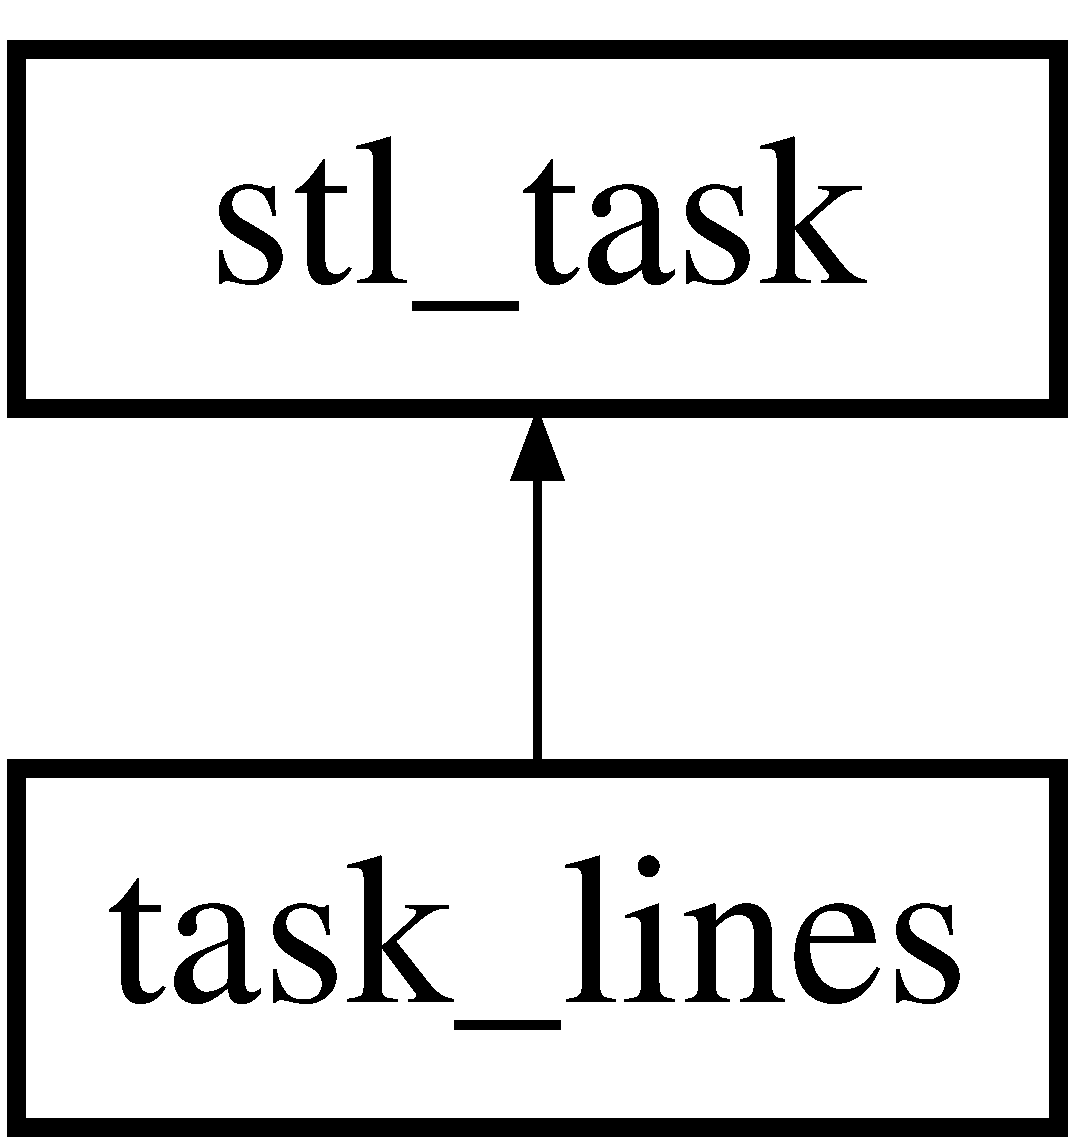
\includegraphics[height=2.000000cm]{classtask__lines}
\end{center}
\end{figure}
\subsection*{Public Member Functions}
\begin{DoxyCompactItemize}
\item 
\hyperlink{classtask__lines_a0d04d45a83ecf3894cdb6c98942e97b6}{task\-\_\-lines} (base\-\_\-text\-\_\-serial $\ast$p\-\_\-serial\-\_\-port, task\-\_\-timer \&a\-\_\-timer, time\-\_\-stamp \&t\-\_\-stamp, \hyperlink{classtask__PID}{task\-\_\-\-P\-I\-D} $\ast$\hyperlink{classtask__lines_af20c4404da342292d6e8e8a7a6004af2}{P\-I\-D\-\_\-1}, \hyperlink{classtask__PID}{task\-\_\-\-P\-I\-D} $\ast$\hyperlink{classtask__lines_ac53057e78b84eeb3576ee7ffb2380981}{P\-I\-D\-\_\-2}, \hyperlink{classpoint}{point} $\ast$get\-\_\-there, \hyperlink{classservo}{servo} $\ast$P\-E\-N)
\item 
char \hyperlink{classtask__lines_adc52a1f1de31103830a06737db769a34}{run} (char)
\item 
\hypertarget{classtask__lines_a58abf21c099eba3afd75e01a41aac160}{void \hyperlink{classtask__lines_a58abf21c099eba3afd75e01a41aac160}{go} (void)}\label{classtask__lines_a58abf21c099eba3afd75e01a41aac160}

\begin{DoxyCompactList}\small\item\em This method sets a bool allowing \hyperlink{classtask__lines}{task\-\_\-lines} to operate. \end{DoxyCompactList}\item 
\hypertarget{classtask__lines_aa4d45fa38ffb509df4587afaf920f5d1}{void \hyperlink{classtask__lines_aa4d45fa38ffb509df4587afaf920f5d1}{set\-\_\-coords} (int16\-\_\-t X0, int16\-\_\-t Y0, int16\-\_\-t X\-\_\-f, int16\-\_\-t Y\-\_\-f)}\label{classtask__lines_aa4d45fa38ffb509df4587afaf920f5d1}

\begin{DoxyCompactList}\small\item\em Set\-\_\-coords updates the initial and final x\&y coordinates when a new line needs to be drawn. \end{DoxyCompactList}\item 
\hypertarget{classtask__lines_a8182baeb4e6d6608bb0b9d5bf7ee02d1}{void \hyperlink{classtask__lines_a8182baeb4e6d6608bb0b9d5bf7ee02d1}{draw\-\_\-signature} (void)}\label{classtask__lines_a8182baeb4e6d6608bb0b9d5bf7ee02d1}

\begin{DoxyCompactList}\small\item\em This method sets up lines to draw our signature. \end{DoxyCompactList}\item 
\hypertarget{classtask__lines_af24660494d5ef22eb6c03a007c7347a1}{bool \hyperlink{classtask__lines_af24660494d5ef22eb6c03a007c7347a1}{wanna\-\_\-go\-\_\-home} (void)}\label{classtask__lines_af24660494d5ef22eb6c03a007c7347a1}

\begin{DoxyCompactList}\small\item\em This method allows \hyperlink{classGo__Home}{Go\-\_\-\-Home} to see if we want to home (after each line). \end{DoxyCompactList}\item 
\hypertarget{classtask__lines_aef4c5d6e9c67d040a398c2d1791e5f19}{void \hyperlink{classtask__lines_aef4c5d6e9c67d040a398c2d1791e5f19}{ok\-\_\-were\-\_\-home} (void)}\label{classtask__lines_aef4c5d6e9c67d040a398c2d1791e5f19}

\begin{DoxyCompactList}\small\item\em This method allows \hyperlink{classGo__Home}{Go\-\_\-\-Home} to lower the homing flag once home is reached. \end{DoxyCompactList}\end{DoxyCompactItemize}
\subsection*{Protected Attributes}
\begin{DoxyCompactItemize}
\item 
\hypertarget{classtask__lines_acdace444a5715561b80dd929aabb6813}{base\-\_\-text\-\_\-serial $\ast$ \hyperlink{classtask__lines_acdace444a5715561b80dd929aabb6813}{ptr\-\_\-2\-\_\-serial}}\label{classtask__lines_acdace444a5715561b80dd929aabb6813}

\begin{DoxyCompactList}\small\item\em pointer to a serial port object for printing purposes \end{DoxyCompactList}\item 
\hypertarget{classtask__lines_adf126ba6072b70e5525f470bc0d5fd90}{\hyperlink{classpoint}{point} $\ast$ \hyperlink{classtask__lines_adf126ba6072b70e5525f470bc0d5fd90}{Initial\-\_\-\-Point}}\label{classtask__lines_adf126ba6072b70e5525f470bc0d5fd90}

\begin{DoxyCompactList}\small\item\em point object used to move machine \end{DoxyCompactList}\item 
\hypertarget{classtask__lines_ac6c15e2f9c29419c3790196ad18b24dd}{\hyperlink{classservo}{servo} $\ast$ \hyperlink{classtask__lines_ac6c15e2f9c29419c3790196ad18b24dd}{operate\-\_\-pen}}\label{classtask__lines_ac6c15e2f9c29419c3790196ad18b24dd}

\begin{DoxyCompactList}\small\item\em servo object used to raise lower pen \end{DoxyCompactList}\item 
\hypertarget{classtask__lines_af20c4404da342292d6e8e8a7a6004af2}{\hyperlink{classtask__PID}{task\-\_\-\-P\-I\-D} $\ast$ \hyperlink{classtask__lines_af20c4404da342292d6e8e8a7a6004af2}{P\-I\-D\-\_\-1}}\label{classtask__lines_af20c4404da342292d6e8e8a7a6004af2}

\begin{DoxyCompactList}\small\item\em P\-I\-D object used to control motor 1. \end{DoxyCompactList}\item 
\hypertarget{classtask__lines_ac53057e78b84eeb3576ee7ffb2380981}{\hyperlink{classtask__PID}{task\-\_\-\-P\-I\-D} $\ast$ \hyperlink{classtask__lines_ac53057e78b84eeb3576ee7ffb2380981}{P\-I\-D\-\_\-2}}\label{classtask__lines_ac53057e78b84eeb3576ee7ffb2380981}

\begin{DoxyCompactList}\small\item\em P\-I\-D object used to control motor 2. \end{DoxyCompactList}\item 
\hypertarget{classtask__lines_a2cb987744a37b733479a1766a61a7734}{bool \hyperlink{classtask__lines_a2cb987744a37b733479a1766a61a7734}{send\-\_\-home}}\label{classtask__lines_a2cb987744a37b733479a1766a61a7734}

\begin{DoxyCompactList}\small\item\em boolean used to request homing \end{DoxyCompactList}\item 
\hypertarget{classtask__lines_a741d9e704cb8842d8b5f18b88c386cb9}{bool \hyperlink{classtask__lines_a741d9e704cb8842d8b5f18b88c386cb9}{divide\-\_\-lines}}\label{classtask__lines_a741d9e704cb8842d8b5f18b88c386cb9}

\begin{DoxyCompactList}\small\item\em boolean which allows lines to begin \end{DoxyCompactList}\item 
\hypertarget{classtask__lines_a7abff223287d4d2e921b71c39bd179ba}{bool \hyperlink{classtask__lines_a7abff223287d4d2e921b71c39bd179ba}{moving}}\label{classtask__lines_a7abff223287d4d2e921b71c39bd179ba}

\begin{DoxyCompactList}\small\item\em boolean used to wait while movement occurs \end{DoxyCompactList}\item 
\hypertarget{classtask__lines_aea9f2c1abc6285bb1131b2098dd2a567}{bool \hyperlink{classtask__lines_aea9f2c1abc6285bb1131b2098dd2a567}{signature}}\label{classtask__lines_aea9f2c1abc6285bb1131b2098dd2a567}

\begin{DoxyCompactList}\small\item\em boolean used to initiate and continue signiture process \end{DoxyCompactList}\item 
\hypertarget{classtask__lines_a67c3830a872bf2d6d2215eec15156e51}{uint8\-\_\-t \hyperlink{classtask__lines_a67c3830a872bf2d6d2215eec15156e51}{sig\-\_\-count}}\label{classtask__lines_a67c3830a872bf2d6d2215eec15156e51}

\begin{DoxyCompactList}\small\item\em sub state variable keeps track of where in signiture we are \end{DoxyCompactList}\item 
\hypertarget{classtask__lines_ae33211839ee44fdf75ba2aef43c8a566}{uint8\-\_\-t \hyperlink{classtask__lines_ae33211839ee44fdf75ba2aef43c8a566}{line\-\_\-type}}\label{classtask__lines_ae33211839ee44fdf75ba2aef43c8a566}

\begin{DoxyCompactList}\small\item\em sub state variable used to transition between line types \end{DoxyCompactList}\item 
\hypertarget{classtask__lines_a90808cf8391311e526bf7a647e499afc}{int8\-\_\-t \hyperlink{classtask__lines_a90808cf8391311e526bf7a647e499afc}{dx}}\label{classtask__lines_a90808cf8391311e526bf7a647e499afc}

\begin{DoxyCompactList}\small\item\em incremental x distance in tenths of an inch \end{DoxyCompactList}\item 
\hypertarget{classtask__lines_a0f086520fb9bfd448685708910d06fe1}{int8\-\_\-t \hyperlink{classtask__lines_a0f086520fb9bfd448685708910d06fe1}{dy}}\label{classtask__lines_a0f086520fb9bfd448685708910d06fe1}

\begin{DoxyCompactList}\small\item\em incremental y distance in tenths of an inch \end{DoxyCompactList}\item 
\hypertarget{classtask__lines_a23ff1336daefdf449e36ae03266dfe0e}{uint16\-\_\-t \hyperlink{classtask__lines_a23ff1336daefdf449e36ae03266dfe0e}{current\-\_\-segment}}\label{classtask__lines_a23ff1336daefdf449e36ae03266dfe0e}

\begin{DoxyCompactList}\small\item\em keeps track of when a line is done \end{DoxyCompactList}\item 
\hypertarget{classtask__lines_aa686a708aa641201a447f31d13a4351b}{uint16\-\_\-t \hyperlink{classtask__lines_aa686a708aa641201a447f31d13a4351b}{Seg\-\_\-\-Total}}\label{classtask__lines_aa686a708aa641201a447f31d13a4351b}

\begin{DoxyCompactList}\small\item\em total number of segments in a line \end{DoxyCompactList}\item 
\hypertarget{classtask__lines_ab160679fe7aa75496e0e4a27789cb6d2}{uint16\-\_\-t \hyperlink{classtask__lines_ab160679fe7aa75496e0e4a27789cb6d2}{counter}}\label{classtask__lines_ab160679fe7aa75496e0e4a27789cb6d2}

\begin{DoxyCompactList}\small\item\em dumb counter used to let pen get down befor next step happens \end{DoxyCompactList}\item 
\hypertarget{classtask__lines_aa7134592021b616761cad2811618aa5c}{int32\-\_\-t \hyperlink{classtask__lines_aa7134592021b616761cad2811618aa5c}{S\-U\-Mdx}}\label{classtask__lines_aa7134592021b616761cad2811618aa5c}

\begin{DoxyCompactList}\small\item\em total change in x \end{DoxyCompactList}\item 
\hypertarget{classtask__lines_a89408d73e8e7a9b53586c55418fd2710}{int32\-\_\-t \hyperlink{classtask__lines_a89408d73e8e7a9b53586c55418fd2710}{S\-U\-Mdy}}\label{classtask__lines_a89408d73e8e7a9b53586c55418fd2710}

\begin{DoxyCompactList}\small\item\em total change in y \end{DoxyCompactList}\item 
\hypertarget{classtask__lines_a4eb29ee98cb4b6a555ddd43804054179}{int16\-\_\-t \hyperlink{classtask__lines_a4eb29ee98cb4b6a555ddd43804054179}{x0}}\label{classtask__lines_a4eb29ee98cb4b6a555ddd43804054179}

\begin{DoxyCompactList}\small\item\em initial x coordinate of a line \end{DoxyCompactList}\item 
\hypertarget{classtask__lines_a0748460c610b0bb8e9cfd8b698206ec1}{int16\-\_\-t \hyperlink{classtask__lines_a0748460c610b0bb8e9cfd8b698206ec1}{y0}}\label{classtask__lines_a0748460c610b0bb8e9cfd8b698206ec1}

\begin{DoxyCompactList}\small\item\em initial y coordinate of a line \end{DoxyCompactList}\item 
\hypertarget{classtask__lines_a13189d18f9ae3bce0e07b23bb9831325}{int16\-\_\-t \hyperlink{classtask__lines_a13189d18f9ae3bce0e07b23bb9831325}{xf}}\label{classtask__lines_a13189d18f9ae3bce0e07b23bb9831325}

\begin{DoxyCompactList}\small\item\em final x coordinate of a line \end{DoxyCompactList}\item 
\hypertarget{classtask__lines_a8cff318f4dc88da0621ba31acbd44d3d}{int16\-\_\-t \hyperlink{classtask__lines_a8cff318f4dc88da0621ba31acbd44d3d}{yf}}\label{classtask__lines_a8cff318f4dc88da0621ba31acbd44d3d}

\begin{DoxyCompactList}\small\item\em final y coordinate of a line \end{DoxyCompactList}\item 
\hypertarget{classtask__lines_a51332b7495541314d657391dcffd6481}{float \hyperlink{classtask__lines_a51332b7495541314d657391dcffd6481}{slope}}\label{classtask__lines_a51332b7495541314d657391dcffd6481}

\begin{DoxyCompactList}\small\item\em to detect lines we can do really well! (through origin) \end{DoxyCompactList}\item 
\hypertarget{classtask__lines_a2d1f5a2952f88bf379e03ec7bdc4b818}{float \hyperlink{classtask__lines_a2d1f5a2952f88bf379e03ec7bdc4b818}{S\-U\-Mx\-\_\-squared}}\label{classtask__lines_a2d1f5a2952f88bf379e03ec7bdc4b818}

\begin{DoxyCompactList}\small\item\em partitioning pythagorean theorum helped math errors stop \end{DoxyCompactList}\item 
\hypertarget{classtask__lines_a1cc6ee26543dbfe85b3500dfdc1712d1}{float \hyperlink{classtask__lines_a1cc6ee26543dbfe85b3500dfdc1712d1}{S\-U\-My\-\_\-squared}}\label{classtask__lines_a1cc6ee26543dbfe85b3500dfdc1712d1}

\begin{DoxyCompactList}\small\item\em partitioning pythagorean theorum helped math errors stop \end{DoxyCompactList}\item 
\hypertarget{classtask__lines_abc0d3f3dbce125e7b35fc116ecf05350}{uint16\-\_\-t \hyperlink{classtask__lines_abc0d3f3dbce125e7b35fc116ecf05350}{S\-U\-Mdx\-\_\-16}}\label{classtask__lines_abc0d3f3dbce125e7b35fc116ecf05350}

\begin{DoxyCompactList}\small\item\em extra variable to help avoid math errors \end{DoxyCompactList}\item 
\hypertarget{classtask__lines_a29bac5ba1aef89204d59be10188508e8}{uint16\-\_\-t \hyperlink{classtask__lines_a29bac5ba1aef89204d59be10188508e8}{S\-U\-Mdy\-\_\-16}}\label{classtask__lines_a29bac5ba1aef89204d59be10188508e8}

\begin{DoxyCompactList}\small\item\em extra variable to help avoid math errors \end{DoxyCompactList}\end{DoxyCompactItemize}


\subsection{Detailed Description}
\hyperlink{task__lines_8cpp}{task\-\_\-lines.\-cpp} is a task which cuts lines into bitty pieces and moves sequentially through the line by moving the setpoint and feeding it to the point task. 

Definition at line 23 of file task\-\_\-lines.\-h.



\subsection{Constructor \& Destructor Documentation}
\hypertarget{classtask__lines_a0d04d45a83ecf3894cdb6c98942e97b6}{\index{task\-\_\-lines@{task\-\_\-lines}!task\-\_\-lines@{task\-\_\-lines}}
\index{task\-\_\-lines@{task\-\_\-lines}!task_lines@{task\-\_\-lines}}
\subsubsection[{task\-\_\-lines}]{\setlength{\rightskip}{0pt plus 5cm}task\-\_\-lines\-::task\-\_\-lines (
\begin{DoxyParamCaption}
\item[{base\-\_\-text\-\_\-serial $\ast$}]{p\-\_\-serial\-\_\-port, }
\item[{task\-\_\-timer \&}]{a\-\_\-timer, }
\item[{time\-\_\-stamp \&}]{t\-\_\-stamp, }
\item[{{\bf task\-\_\-\-P\-I\-D} $\ast$}]{motor\-\_\-1, }
\item[{{\bf task\-\_\-\-P\-I\-D} $\ast$}]{motor\-\_\-2, }
\item[{{\bf point} $\ast$}]{get\-\_\-there, }
\item[{{\bf servo} $\ast$}]{P\-E\-N}
\end{DoxyParamCaption}
)}}\label{classtask__lines_a0d04d45a83ecf3894cdb6c98942e97b6}
The constructor initializes variables, and saves object pointers locally. 
\begin{DoxyParams}{Parameters}
{\em p\-\_\-serial\-\_\-port} & Serial object so we can write to screen \\
\hline
{\em a\-\_\-timer} & Time value used for S\-T\-L scheduling \\
\hline
{\em t\-\_\-stamp} & Time stamp used for S\-T\-L scheduling \\
\hline
{\em motor\-\_\-1} & P\-I\-D object for motor 1 \\
\hline
{\em motor\-\_\-2} & P\-I\-D object for motor 2 \\
\hline
{\em get\-\_\-there} & Point object used to move from setpoint to setpoint \\
\hline
{\em P\-E\-N} & Servo Object to raise/lower pen \\
\hline
\end{DoxyParams}


Definition at line 45 of file task\-\_\-lines.\-cpp.



References divide\-\_\-lines, Initial\-\_\-\-Point, moving, operate\-\_\-pen, P\-I\-D\-\_\-1, P\-I\-D\-\_\-2, ptr\-\_\-2\-\_\-serial, send\-\_\-home, sig\-\_\-count, signature, x0, xf, y0, and yf.



\subsection{Member Function Documentation}
\hypertarget{classtask__lines_adc52a1f1de31103830a06737db769a34}{\index{task\-\_\-lines@{task\-\_\-lines}!run@{run}}
\index{run@{run}!task_lines@{task\-\_\-lines}}
\subsubsection[{run}]{\setlength{\rightskip}{0pt plus 5cm}char task\-\_\-lines\-::run (
\begin{DoxyParamCaption}
\item[{char}]{state}
\end{DoxyParamCaption}
)}}\label{classtask__lines_adc52a1f1de31103830a06737db769a34}
run is the main method in \hyperlink{classtask__lines}{task\-\_\-lines}. It takes care of the math involved in cutting a line into segments. It first takes the initial and final x\&y coordinates, uses the pythagorean theorem to find the length of the actual line, determins how many segments to break the line up into based on it's overall length, calculates the slope of the line, and then uses the slope along with the change in the x\&y coordinates to determine if the line passes through the origin (type 1), is vertical (type 2), is horizontal (type 4), or general and none of the above (type 3). The reason for categorizing what type of line you're drawing is because the algorithm is slightly different for each line type and certain lines can be drawn much faster by using a different algorithm, especially lines which pass through the origin. \hyperlink{classtask__lines}{task\-\_\-lines} then breaks the line into smaller segments, keeps track of what segment the polar plotter is currently on, increments setpoints as each one is reached, and uses the point object to physically move the pen to the next setpoint. All of this is accomplished using a switch-\/case structure and flags which are raised and lowered depending on what needs to happen. 
\begin{DoxyParams}{Parameters}
{\em state} & This method uses S\-T\-L\-\_\-task to transition its state \\
\hline
\end{DoxyParams}
State 0 is a wait state. Is a new line requested?

State 1 does some initial x-\/y to r-\/theta calculations

State 2 starts movement towards initial point

State 3 waits for attainment of initial point

state 4 draws line which would pass through origin

state 5 draws vertical lines

state 6 draws general lines

state 7 draws horizontal lines

State 8 draws our signature!

State 9 sends the plotter home after each line in our signature 

Definition at line 81 of file task\-\_\-lines.\-cpp.



References point\-::\-Are\-\_\-\-We\-\_\-\-There(), counter, current\-\_\-segment, divide\-\_\-lines, dx, dy, servo\-::\-Fine\-\_\-\-Line(), point\-::\-Get\-\_\-\-There(), Initial\-\_\-\-Point, line\-\_\-type, moving, operate\-\_\-pen, servo\-::\-Pen\-\_\-\-Up(), P\-I\-D\-\_\-1, P\-I\-D\-\_\-2, Seg\-\_\-\-Total, send\-\_\-home, set\-\_\-coords(), sig\-\_\-count, signature, slope, task\-\_\-\-P\-I\-D\-::stop(), S\-U\-Mdx, S\-U\-Mdx\-\_\-16, S\-U\-Mdy, S\-U\-Mdy\-\_\-16, S\-U\-Mx\-\_\-squared, S\-U\-My\-\_\-squared, x0, xf, y0, and yf.



The documentation for this class was generated from the following files\-:\begin{DoxyCompactItemize}
\item 
\hyperlink{task__lines_8h}{task\-\_\-lines.\-h}\item 
\hyperlink{task__lines_8cpp}{task\-\_\-lines.\-cpp}\end{DoxyCompactItemize}

\hypertarget{classtask__PID}{\section{task\-\_\-\-P\-I\-D Class Reference}
\label{classtask__PID}\index{task\-\_\-\-P\-I\-D@{task\-\_\-\-P\-I\-D}}
}


{\ttfamily \#include $<$task\-\_\-\-P\-I\-D.\-h$>$}

Inheritance diagram for task\-\_\-\-P\-I\-D\-:\begin{figure}[H]
\begin{center}
\leavevmode
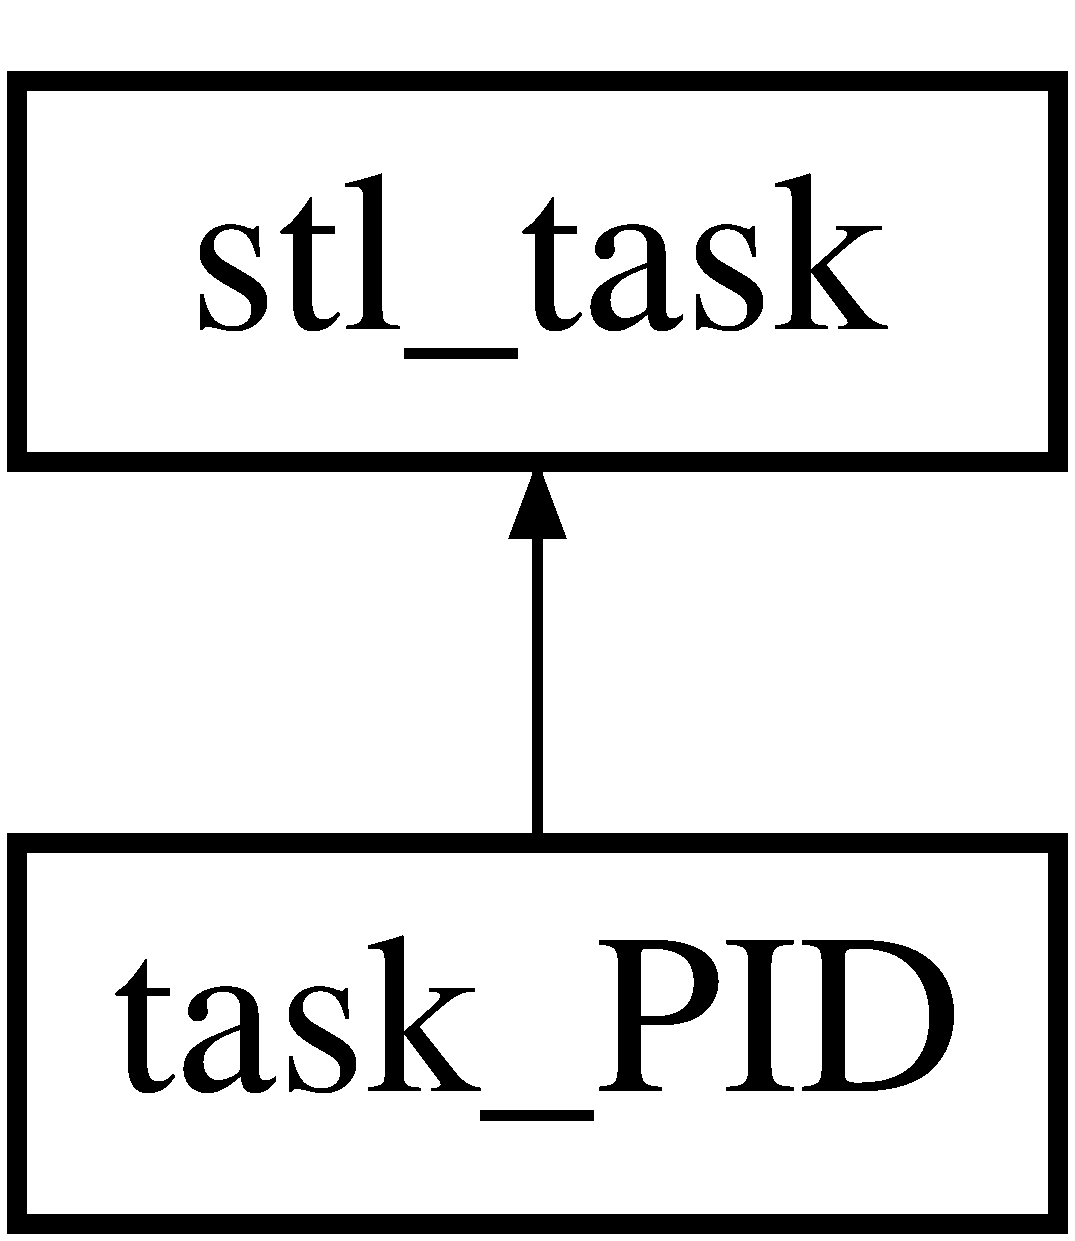
\includegraphics[height=2.000000cm]{classtask__PID}
\end{center}
\end{figure}
\subsection*{Public Member Functions}
\begin{DoxyCompactItemize}
\item 
\hyperlink{classtask__PID_a2e6f07f6c2d77478c31098a329c0e145}{task\-\_\-\-P\-I\-D} (base\-\_\-text\-\_\-serial $\ast$p\-\_\-serial\-\_\-port, task\-\_\-timer \&a\-\_\-timer, time\-\_\-stamp \&t\-\_\-stamp, \hyperlink{classMaster}{Master} $\ast$master\-\_\-object, \hyperlink{classda__motor}{da\-\_\-motor} $\ast$motor\-\_\-object, uint8\-\_\-t which\-\_\-\-Channel)
\item 
char \hyperlink{classtask__PID_a6f05dcd8d4efe5ab56610e02ea814b7b}{run} (char)
\item 
void \hyperlink{classtask__PID_af5c32248046e469d4a7d84bf5edef147}{go} (void)
\item 
void \hyperlink{classtask__PID_af0a7b8ea266e97a883b58a8efc7812e4}{stop} (void)
\item 
void \hyperlink{classtask__PID_a39f37fa8c4514697bc6fe25fc6bd3498}{C\-L\-E\-A\-R} (void)
\item 
void \hyperlink{classtask__PID_a42c0117a576e25c264e2d62c6224ba6f}{set\-\_\-kp} (uint16\-\_\-t kp\-\_\-val)
\begin{DoxyCompactList}\small\item\em set K\-\_\-p \end{DoxyCompactList}\item 
void \hyperlink{classtask__PID_a6b61639ae796073f60e452a19a692e4e}{set\-\_\-ki} (uint16\-\_\-t ki\-\_\-val)
\begin{DoxyCompactList}\small\item\em set K\-\_\-i \end{DoxyCompactList}\item 
void \hyperlink{classtask__PID_ab086212c737d28bfa3af6f423eb4c54a}{set\-\_\-kd} (uint16\-\_\-t kd\-\_\-val)
\begin{DoxyCompactList}\small\item\em set K\-\_\-d \end{DoxyCompactList}\item 
\hypertarget{classtask__PID_ae4dbe31628ed6557e7703494006744e4}{uint16\-\_\-t \hyperlink{classtask__PID_ae4dbe31628ed6557e7703494006744e4}{G\-E\-T\-\_\-\-Kp} (void)}\label{classtask__PID_ae4dbe31628ed6557e7703494006744e4}

\begin{DoxyCompactList}\small\item\em G\-E\-T\-\_\-\-Kp returns K\-\_\-p. \end{DoxyCompactList}\item 
\hypertarget{classtask__PID_a3e065d324a3f296cf32297370a6026c4}{uint16\-\_\-t \hyperlink{classtask__PID_a3e065d324a3f296cf32297370a6026c4}{G\-E\-T\-\_\-\-Ki} (void)}\label{classtask__PID_a3e065d324a3f296cf32297370a6026c4}

\begin{DoxyCompactList}\small\item\em G\-E\-T\-\_\-\-Ki returns K\-\_\-i. \end{DoxyCompactList}\item 
\hypertarget{classtask__PID_a5ed698383876a6968310bac2f70f78f9}{uint16\-\_\-t \hyperlink{classtask__PID_a5ed698383876a6968310bac2f70f78f9}{G\-E\-T\-\_\-\-Kd} (void)}\label{classtask__PID_a5ed698383876a6968310bac2f70f78f9}

\begin{DoxyCompactList}\small\item\em G\-E\-T\-\_\-\-Kd returns K\-\_\-d. \end{DoxyCompactList}\item 
void \hyperlink{classtask__PID_a5112215d3f09f07c8269724417b81232}{set\-\_\-setpoint} (int32\-\_\-t s\-\_\-pt)
\item 
int32\-\_\-t \hyperlink{classtask__PID_abb3876eab56d800fa45d99b77d0fed40}{G\-E\-T\-\_\-setpoint} (void)
\item 
int32\-\_\-t \hyperlink{classtask__PID_a3df066e30232d9262cffe00a209aa838}{Get\-\_\-\-Encoder} (void)
\item 
bool \hyperlink{classtask__PID_abb2aa5643b7c4909d930dfb281a6eaa2}{At\-\_\-\-Seg\-\_\-\-End} (void)
\item 
void \hyperlink{classtask__PID_a5d79acbd155902dc1a10d1968f4c6050}{Request\-\_\-\-Home} (bool Nice\-\_\-\-Shoes)
\end{DoxyCompactItemize}
\subsection*{Protected Attributes}
\begin{DoxyCompactItemize}
\item 
\hypertarget{classtask__PID_abb3ce7591adb11f5dfaf185a60783079}{base\-\_\-text\-\_\-serial $\ast$ \hyperlink{classtask__PID_abb3ce7591adb11f5dfaf185a60783079}{ptr\-\_\-2\-\_\-serial}}\label{classtask__PID_abb3ce7591adb11f5dfaf185a60783079}

\begin{DoxyCompactList}\small\item\em pointer to a serial port object for printing purposes \end{DoxyCompactList}\item 
\hypertarget{classtask__PID_a8ed91ccc6f7ce2161f82911fafd35a2b}{\hyperlink{classMaster}{Master} $\ast$ \hyperlink{classtask__PID_a8ed91ccc6f7ce2161f82911fafd35a2b}{func\-\_\-\-R\-E\-A\-D\-\_\-\-E\-N\-C\-O\-D\-E\-R}}\label{classtask__PID_a8ed91ccc6f7ce2161f82911fafd35a2b}

\begin{DoxyCompactList}\small\item\em pointer of type \hyperlink{classMaster}{Master} to an S\-P\-I object \end{DoxyCompactList}\item 
\hypertarget{classtask__PID_a3b21278136079ae694190e3f620c40cf}{\hyperlink{classda__motor}{da\-\_\-motor} $\ast$ \hyperlink{classtask__PID_a3b21278136079ae694190e3f620c40cf}{func\-\_\-\-U\-P\-D\-A\-T\-E\-\_\-\-M\-O\-T\-O\-R}}\label{classtask__PID_a3b21278136079ae694190e3f620c40cf}

\begin{DoxyCompactList}\small\item\em pointer of type \hyperlink{classda__motor}{da\-\_\-motor} to a motor object \end{DoxyCompactList}\item 
\hypertarget{classtask__PID_a4db9c3da4224504ff3689ad2e16eeeab}{bool \hyperlink{classtask__PID_a4db9c3da4224504ff3689ad2e16eeeab}{giddyup}}\label{classtask__PID_a4db9c3da4224504ff3689ad2e16eeeab}

\begin{DoxyCompactList}\small\item\em tell motor to stop or go \end{DoxyCompactList}\item 
\hypertarget{classtask__PID_a89911b07245fec5c4403f9f781f02788}{bool \hyperlink{classtask__PID_a89911b07245fec5c4403f9f781f02788}{homing}}\label{classtask__PID_a89911b07245fec5c4403f9f781f02788}

\begin{DoxyCompactList}\small\item\em homing allows task \hyperlink{classGo__Home}{Go\-\_\-\-Home} to take control of motors \end{DoxyCompactList}\item 
\hypertarget{classtask__PID_aabeac3edf9b1dc94f9e216ab99d89798}{uint8\-\_\-t \hyperlink{classtask__PID_aabeac3edf9b1dc94f9e216ab99d89798}{motor\-\_\-num}}\label{classtask__PID_aabeac3edf9b1dc94f9e216ab99d89798}

\begin{DoxyCompactList}\small\item\em a constant for each P\-I\-D which controls which motor and encoder we use each time the P\-I\-D is called \end{DoxyCompactList}\item 
\hypertarget{classtask__PID_a3aad6e651da5110ea8d64971272d611b}{uint8\-\_\-t \hyperlink{classtask__PID_a3aad6e651da5110ea8d64971272d611b}{Checksum\-\_\-\-Error\-\_\-flag}}\label{classtask__PID_a3aad6e651da5110ea8d64971272d611b}

\begin{DoxyCompactList}\small\item\em A flag which indicates an S\-P\-I transfer error. \end{DoxyCompactList}\item 
\hypertarget{classtask__PID_a40708de7482ae8000f09de573757b763}{volatile uint8\-\_\-t \hyperlink{classtask__PID_a40708de7482ae8000f09de573757b763}{dummy}}\label{classtask__PID_a40708de7482ae8000f09de573757b763}

\begin{DoxyCompactList}\small\item\em stupid counting variable \end{DoxyCompactList}\item 
\hypertarget{classtask__PID_a0ed9811d402294a2e97513d17603cbde}{uint8\-\_\-t \hyperlink{classtask__PID_a0ed9811d402294a2e97513d17603cbde}{duty\-\_\-cycle}}\label{classtask__PID_a0ed9811d402294a2e97513d17603cbde}

\begin{DoxyCompactList}\small\item\em name pretty well says it \end{DoxyCompactList}\item 
\hypertarget{classtask__PID_a819c45f7b06d30c0c259434e519920df}{uint16\-\_\-t \hyperlink{classtask__PID_a819c45f7b06d30c0c259434e519920df}{K\-\_\-p}}\label{classtask__PID_a819c45f7b06d30c0c259434e519920df}

\begin{DoxyCompactList}\small\item\em proportional gain \end{DoxyCompactList}\item 
\hypertarget{classtask__PID_abdd29e3d3a304269e80c9a8008f23a27}{uint16\-\_\-t \hyperlink{classtask__PID_abdd29e3d3a304269e80c9a8008f23a27}{K\-\_\-i}}\label{classtask__PID_abdd29e3d3a304269e80c9a8008f23a27}

\begin{DoxyCompactList}\small\item\em integral gain \end{DoxyCompactList}\item 
\hypertarget{classtask__PID_a6aff3da930aa2bab02ecc480682653b7}{uint16\-\_\-t \hyperlink{classtask__PID_a6aff3da930aa2bab02ecc480682653b7}{K\-\_\-d}}\label{classtask__PID_a6aff3da930aa2bab02ecc480682653b7}

\begin{DoxyCompactList}\small\item\em differential gain \end{DoxyCompactList}\item 
\hypertarget{classtask__PID_abc82ee4ac88e8eae7d3ec15a980c07aa}{int32\-\_\-t \hyperlink{classtask__PID_abc82ee4ac88e8eae7d3ec15a980c07aa}{prev\-\_\-error}}\label{classtask__PID_abc82ee4ac88e8eae7d3ec15a980c07aa}

\begin{DoxyCompactList}\small\item\em used for differential feedback \end{DoxyCompactList}\item 
\hypertarget{classtask__PID_a788dfa787dc2ca005f59a33bc844ffc8}{int32\-\_\-t \hyperlink{classtask__PID_a788dfa787dc2ca005f59a33bc844ffc8}{E\-\_\-sum\-\_\-old}}\label{classtask__PID_a788dfa787dc2ca005f59a33bc844ffc8}

\begin{DoxyCompactList}\small\item\em used for integral feedback \end{DoxyCompactList}\item 
\hypertarget{classtask__PID_a174d94530691e307bcbbf39f33b67650}{int32\-\_\-t \hyperlink{classtask__PID_a174d94530691e307bcbbf39f33b67650}{encoder}}\label{classtask__PID_a174d94530691e307bcbbf39f33b67650}

\begin{DoxyCompactList}\small\item\em encoder reading \end{DoxyCompactList}\item 
\hypertarget{classtask__PID_a40baac51f6290267531fd27550124543}{int32\-\_\-t \hyperlink{classtask__PID_a40baac51f6290267531fd27550124543}{Set\-\_\-\-Point}}\label{classtask__PID_a40baac51f6290267531fd27550124543}

\begin{DoxyCompactList}\small\item\em the set point \end{DoxyCompactList}\item 
\hypertarget{classtask__PID_a9d046f072b58189aed139ea63d853fd4}{bool \hyperlink{classtask__PID_a9d046f072b58189aed139ea63d853fd4}{are\-\_\-we\-\_\-there\-\_\-yet}}\label{classtask__PID_a9d046f072b58189aed139ea63d853fd4}

\begin{DoxyCompactList}\small\item\em boolean set to true when desired position is reached \end{DoxyCompactList}\end{DoxyCompactItemize}


\subsection{Detailed Description}
\hyperlink{task__PID_8cpp}{task\-\_\-\-P\-I\-D.\-cpp} is a class for a P\-I\-D controller. \hyperlink{classtask__PID}{task\-\_\-\-P\-I\-D} is able to read the current encoder position on a motor, calculate the proportional, integral, and differential gains, and update the motor's duty cycle based on the final gain value. It can also manipulate certain flags via inline functions to trigger actions, such as telling a motor to go or stop, in other objects. 

Definition at line 22 of file task\-\_\-\-P\-I\-D.\-h.



\subsection{Constructor \& Destructor Documentation}
\hypertarget{classtask__PID_a2e6f07f6c2d77478c31098a329c0e145}{\index{task\-\_\-\-P\-I\-D@{task\-\_\-\-P\-I\-D}!task\-\_\-\-P\-I\-D@{task\-\_\-\-P\-I\-D}}
\index{task\-\_\-\-P\-I\-D@{task\-\_\-\-P\-I\-D}!task_PID@{task\-\_\-\-P\-I\-D}}
\subsubsection[{task\-\_\-\-P\-I\-D}]{\setlength{\rightskip}{0pt plus 5cm}task\-\_\-\-P\-I\-D\-::task\-\_\-\-P\-I\-D (
\begin{DoxyParamCaption}
\item[{base\-\_\-text\-\_\-serial $\ast$}]{p\-\_\-serial\-\_\-port, }
\item[{task\-\_\-timer \&}]{a\-\_\-timer, }
\item[{time\-\_\-stamp \&}]{t\-\_\-stamp, }
\item[{{\bf Master} $\ast$}]{master\-\_\-object, }
\item[{{\bf da\-\_\-motor} $\ast$}]{motor\-\_\-object, }
\item[{uint8\-\_\-t}]{Which\-\_\-\-Channel}
\end{DoxyParamCaption}
)}}\label{classtask__PID_a2e6f07f6c2d77478c31098a329c0e145}
The constructor \hyperlink{classtask__PID}{task\-\_\-\-P\-I\-D} creates a new P\-I\-D object. 
\begin{DoxyParams}{Parameters}
{\em p\-\_\-serial\-\_\-port} & Allows screen printouts \\
\hline
{\em a\-\_\-timer,\-:} & Assists in sceduling \\
\hline
{\em t\-\_\-stamp,\-:} & Assists in sceduling \\
\hline
{\em master\-\_\-object} & An S\-P\-I master object \\
\hline
{\em motor\-\_\-object,\-:} & A motor object \\
\hline
{\em Which\-\_\-\-Channel,\-:} & Gives the newborn P\-I\-D its motor assignment. For life.\\
\hline
\end{DoxyParams}
The constructor \hyperlink{classtask__PID}{task\-\_\-\-P\-I\-D} creates a new Proportional Integral Differential (P\-I\-D) controller object. 
\begin{DoxyParams}{Parameters}
{\em p\-\_\-serial\-\_\-port} & Allows screen printouts \\
\hline
{\em a\-\_\-timer,\-:} & Assists in sceduling \\
\hline
{\em t\-\_\-stamp,\-:} & Assists in sceduling \\
\hline
{\em master\-\_\-object} & An S\-P\-I master object \\
\hline
{\em motor\-\_\-object,\-:} & A motor object \\
\hline
{\em Which\-\_\-\-Channel,\-:} & Gives the newborn P\-I\-D its motor assignment. For life. \\
\hline
\end{DoxyParams}


Definition at line 40 of file task\-\_\-\-P\-I\-D.\-cpp.



References are\-\_\-we\-\_\-there\-\_\-yet, duty\-\_\-cycle, E\-\_\-sum\-\_\-old, encoder, func\-\_\-\-R\-E\-A\-D\-\_\-\-E\-N\-C\-O\-D\-E\-R, func\-\_\-\-U\-P\-D\-A\-T\-E\-\_\-\-M\-O\-T\-O\-R, giddyup, homing, K\-\_\-d, K\-\_\-i, K\-\_\-p, motor\-\_\-num, prev\-\_\-error, ptr\-\_\-2\-\_\-serial, and Set\-\_\-\-Point.



\subsection{Member Function Documentation}
\hypertarget{classtask__PID_abb2aa5643b7c4909d930dfb281a6eaa2}{\index{task\-\_\-\-P\-I\-D@{task\-\_\-\-P\-I\-D}!At\-\_\-\-Seg\-\_\-\-End@{At\-\_\-\-Seg\-\_\-\-End}}
\index{At\-\_\-\-Seg\-\_\-\-End@{At\-\_\-\-Seg\-\_\-\-End}!task_PID@{task\-\_\-\-P\-I\-D}}
\subsubsection[{At\-\_\-\-Seg\-\_\-\-End}]{\setlength{\rightskip}{0pt plus 5cm}bool task\-\_\-\-P\-I\-D\-::\-At\-\_\-\-Seg\-\_\-\-End (
\begin{DoxyParamCaption}
\item[{void}]{}
\end{DoxyParamCaption}
)\hspace{0.3cm}{\ttfamily [inline]}}}\label{classtask__PID_abb2aa5643b7c4909d930dfb281a6eaa2}
check if we're at the end of the segment 

Definition at line 117 of file task\-\_\-\-P\-I\-D.\-h.



References are\-\_\-we\-\_\-there\-\_\-yet.



Referenced by point\-::run().

\hypertarget{classtask__PID_a39f37fa8c4514697bc6fe25fc6bd3498}{\index{task\-\_\-\-P\-I\-D@{task\-\_\-\-P\-I\-D}!C\-L\-E\-A\-R@{C\-L\-E\-A\-R}}
\index{C\-L\-E\-A\-R@{C\-L\-E\-A\-R}!task_PID@{task\-\_\-\-P\-I\-D}}
\subsubsection[{C\-L\-E\-A\-R}]{\setlength{\rightskip}{0pt plus 5cm}void task\-\_\-\-P\-I\-D\-::\-C\-L\-E\-A\-R (
\begin{DoxyParamCaption}
\item[{void}]{}
\end{DoxyParamCaption}
)}}\label{classtask__PID_a39f37fa8c4514697bc6fe25fc6bd3498}
C\-L\-E\-A\-R resets P\-I\-D control variables 

Definition at line 192 of file task\-\_\-\-P\-I\-D.\-cpp.



References duty\-\_\-cycle, E\-\_\-sum\-\_\-old, encoder, and prev\-\_\-error.



Referenced by Go\-\_\-\-Home\-::run().

\hypertarget{classtask__PID_a3df066e30232d9262cffe00a209aa838}{\index{task\-\_\-\-P\-I\-D@{task\-\_\-\-P\-I\-D}!Get\-\_\-\-Encoder@{Get\-\_\-\-Encoder}}
\index{Get\-\_\-\-Encoder@{Get\-\_\-\-Encoder}!task_PID@{task\-\_\-\-P\-I\-D}}
\subsubsection[{Get\-\_\-\-Encoder}]{\setlength{\rightskip}{0pt plus 5cm}int32\-\_\-t task\-\_\-\-P\-I\-D\-::\-Get\-\_\-\-Encoder (
\begin{DoxyParamCaption}
\item[{void}]{}
\end{DoxyParamCaption}
)\hspace{0.3cm}{\ttfamily [inline]}}}\label{classtask__PID_a3df066e30232d9262cffe00a209aa838}
Get\-\_\-\-Encoder gets an encoder reading 

Definition at line 113 of file task\-\_\-\-P\-I\-D.\-h.



References encoder.



Referenced by run().

\hypertarget{classtask__PID_abb3876eab56d800fa45d99b77d0fed40}{\index{task\-\_\-\-P\-I\-D@{task\-\_\-\-P\-I\-D}!G\-E\-T\-\_\-setpoint@{G\-E\-T\-\_\-setpoint}}
\index{G\-E\-T\-\_\-setpoint@{G\-E\-T\-\_\-setpoint}!task_PID@{task\-\_\-\-P\-I\-D}}
\subsubsection[{G\-E\-T\-\_\-setpoint}]{\setlength{\rightskip}{0pt plus 5cm}int32\-\_\-t task\-\_\-\-P\-I\-D\-::\-G\-E\-T\-\_\-setpoint (
\begin{DoxyParamCaption}
\item[{void}]{}
\end{DoxyParamCaption}
)\hspace{0.3cm}{\ttfamily [inline]}}}\label{classtask__PID_abb3876eab56d800fa45d99b77d0fed40}
G\-E\-T\-\_\-setpoint gets the current setpoint so it can be printed 
\begin{DoxyParams}{Parameters}
{\em Set\-\_\-\-Point} & the set point you desire \\
\hline
\end{DoxyParams}


Definition at line 109 of file task\-\_\-\-P\-I\-D.\-h.



References Set\-\_\-\-Point.

\hypertarget{classtask__PID_af5c32248046e469d4a7d84bf5edef147}{\index{task\-\_\-\-P\-I\-D@{task\-\_\-\-P\-I\-D}!go@{go}}
\index{go@{go}!task_PID@{task\-\_\-\-P\-I\-D}}
\subsubsection[{go}]{\setlength{\rightskip}{0pt plus 5cm}void task\-\_\-\-P\-I\-D\-::go (
\begin{DoxyParamCaption}
\item[{void}]{}
\end{DoxyParamCaption}
)}}\label{classtask__PID_af5c32248046e469d4a7d84bf5edef147}
go enables motor control 

Definition at line 177 of file task\-\_\-\-P\-I\-D.\-cpp.



References are\-\_\-we\-\_\-there\-\_\-yet, and giddyup.



Referenced by point\-::run().

\hypertarget{classtask__PID_a5d79acbd155902dc1a10d1968f4c6050}{\index{task\-\_\-\-P\-I\-D@{task\-\_\-\-P\-I\-D}!Request\-\_\-\-Home@{Request\-\_\-\-Home}}
\index{Request\-\_\-\-Home@{Request\-\_\-\-Home}!task_PID@{task\-\_\-\-P\-I\-D}}
\subsubsection[{Request\-\_\-\-Home}]{\setlength{\rightskip}{0pt plus 5cm}void task\-\_\-\-P\-I\-D\-::\-Request\-\_\-\-Home (
\begin{DoxyParamCaption}
\item[{bool}]{Nice\-\_\-\-Shoes}
\end{DoxyParamCaption}
)\hspace{0.3cm}{\ttfamily [inline]}}}\label{classtask__PID_a5d79acbd155902dc1a10d1968f4c6050}
disable P\-I\-D so homing can occur 
\begin{DoxyParams}{Parameters}
{\em Nice\-\_\-\-Shoes} & set this true to disable P\-I\-D for homing \\
\hline
\end{DoxyParams}


Definition at line 122 of file task\-\_\-\-P\-I\-D.\-h.



References homing.



Referenced by Go\-\_\-\-Home\-::run(), and task\-\_\-read\-::run().

\hypertarget{classtask__PID_a6f05dcd8d4efe5ab56610e02ea814b7b}{\index{task\-\_\-\-P\-I\-D@{task\-\_\-\-P\-I\-D}!run@{run}}
\index{run@{run}!task_PID@{task\-\_\-\-P\-I\-D}}
\subsubsection[{run}]{\setlength{\rightskip}{0pt plus 5cm}char task\-\_\-\-P\-I\-D\-::run (
\begin{DoxyParamCaption}
\item[{char}]{state}
\end{DoxyParamCaption}
)}}\label{classtask__PID_a6f05dcd8d4efe5ab56610e02ea814b7b}
run is a 2 state P\-I\-D controller. State 0 is an idle state which wits for the go bool giddyup to be true. State 1 gets an encoder count, does necessary feedback calculations and sets motor duty cycle. 
\begin{DoxyParams}{Parameters}
{\em state} & is a state variable controlled by S\-T\-L\-\_\-task\\
\hline
\end{DoxyParams}
run is a two state P\-I\-D controller. The first state is simply a non moving state which checks to see if movement has been requested. State two incorporates proportional, integral and differential feedback into a control loop which updates the duty cycle of a motor (one motor per P\-I\-D object). State 0 is a non moving state. It doesn't move.

State 1 is the P\-I\-D task. It gets a current encoder reading (ensuring no transfer error) and then calculates new duty and sets the duty cycle.

Definition at line 72 of file task\-\_\-\-P\-I\-D.\-cpp.



References are\-\_\-we\-\_\-there\-\_\-yet, Checksum\-\_\-\-Error\-\_\-flag, dummy, duty\-\_\-cycle, E\-\_\-sum\-\_\-old, encoder, func\-\_\-\-R\-E\-A\-D\-\_\-\-E\-N\-C\-O\-D\-E\-R, func\-\_\-\-U\-P\-D\-A\-T\-E\-\_\-\-M\-O\-T\-O\-R, Get\-\_\-\-Encoder(), giddyup, homing, K\-\_\-i, K\-\_\-p, motor\-\_\-num, prev\-\_\-error, da\-\_\-motor\-::set\-\_\-mode(), Set\-\_\-\-Point, and da\-\_\-motor\-::update\-\_\-duty\-\_\-cycle().

\hypertarget{classtask__PID_ab086212c737d28bfa3af6f423eb4c54a}{\index{task\-\_\-\-P\-I\-D@{task\-\_\-\-P\-I\-D}!set\-\_\-kd@{set\-\_\-kd}}
\index{set\-\_\-kd@{set\-\_\-kd}!task_PID@{task\-\_\-\-P\-I\-D}}
\subsubsection[{set\-\_\-kd}]{\setlength{\rightskip}{0pt plus 5cm}void task\-\_\-\-P\-I\-D\-::set\-\_\-kd (
\begin{DoxyParamCaption}
\item[{uint16\-\_\-t}]{kd\-\_\-val}
\end{DoxyParamCaption}
)\hspace{0.3cm}{\ttfamily [inline]}}}\label{classtask__PID_ab086212c737d28bfa3af6f423eb4c54a}


set K\-\_\-d 


\begin{DoxyParams}{Parameters}
{\em kd\-\_\-val,\-:} & the value you wish to set the gain to \\
\hline
\end{DoxyParams}


Definition at line 91 of file task\-\_\-\-P\-I\-D.\-h.



References K\-\_\-d.

\hypertarget{classtask__PID_a6b61639ae796073f60e452a19a692e4e}{\index{task\-\_\-\-P\-I\-D@{task\-\_\-\-P\-I\-D}!set\-\_\-ki@{set\-\_\-ki}}
\index{set\-\_\-ki@{set\-\_\-ki}!task_PID@{task\-\_\-\-P\-I\-D}}
\subsubsection[{set\-\_\-ki}]{\setlength{\rightskip}{0pt plus 5cm}void task\-\_\-\-P\-I\-D\-::set\-\_\-ki (
\begin{DoxyParamCaption}
\item[{uint16\-\_\-t}]{ki\-\_\-val}
\end{DoxyParamCaption}
)\hspace{0.3cm}{\ttfamily [inline]}}}\label{classtask__PID_a6b61639ae796073f60e452a19a692e4e}


set K\-\_\-i 


\begin{DoxyParams}{Parameters}
{\em ki\-\_\-val,\-:} & the value you wish to set the gain to \\
\hline
\end{DoxyParams}


Definition at line 89 of file task\-\_\-\-P\-I\-D.\-h.



References K\-\_\-i.

\hypertarget{classtask__PID_a42c0117a576e25c264e2d62c6224ba6f}{\index{task\-\_\-\-P\-I\-D@{task\-\_\-\-P\-I\-D}!set\-\_\-kp@{set\-\_\-kp}}
\index{set\-\_\-kp@{set\-\_\-kp}!task_PID@{task\-\_\-\-P\-I\-D}}
\subsubsection[{set\-\_\-kp}]{\setlength{\rightskip}{0pt plus 5cm}void task\-\_\-\-P\-I\-D\-::set\-\_\-kp (
\begin{DoxyParamCaption}
\item[{uint16\-\_\-t}]{kp\-\_\-val}
\end{DoxyParamCaption}
)\hspace{0.3cm}{\ttfamily [inline]}}}\label{classtask__PID_a42c0117a576e25c264e2d62c6224ba6f}


set K\-\_\-p 


\begin{DoxyParams}{Parameters}
{\em kp\-\_\-val,\-:} & the value you wish to set the gain to \\
\hline
\end{DoxyParams}


Definition at line 87 of file task\-\_\-\-P\-I\-D.\-h.



References K\-\_\-p.

\hypertarget{classtask__PID_a5112215d3f09f07c8269724417b81232}{\index{task\-\_\-\-P\-I\-D@{task\-\_\-\-P\-I\-D}!set\-\_\-setpoint@{set\-\_\-setpoint}}
\index{set\-\_\-setpoint@{set\-\_\-setpoint}!task_PID@{task\-\_\-\-P\-I\-D}}
\subsubsection[{set\-\_\-setpoint}]{\setlength{\rightskip}{0pt plus 5cm}void task\-\_\-\-P\-I\-D\-::set\-\_\-setpoint (
\begin{DoxyParamCaption}
\item[{int32\-\_\-t}]{s\-\_\-pt}
\end{DoxyParamCaption}
)\hspace{0.3cm}{\ttfamily [inline]}}}\label{classtask__PID_a5112215d3f09f07c8269724417b81232}
set\-\_\-setpoint sets the setpoint 
\begin{DoxyParams}{Parameters}
{\em s\-\_\-pt} & the set point you desire \\
\hline
\end{DoxyParams}


Definition at line 104 of file task\-\_\-\-P\-I\-D.\-h.



References are\-\_\-we\-\_\-there\-\_\-yet, and Set\-\_\-\-Point.



Referenced by point\-::run().

\hypertarget{classtask__PID_af0a7b8ea266e97a883b58a8efc7812e4}{\index{task\-\_\-\-P\-I\-D@{task\-\_\-\-P\-I\-D}!stop@{stop}}
\index{stop@{stop}!task_PID@{task\-\_\-\-P\-I\-D}}
\subsubsection[{stop}]{\setlength{\rightskip}{0pt plus 5cm}void task\-\_\-\-P\-I\-D\-::stop (
\begin{DoxyParamCaption}
\item[{void}]{}
\end{DoxyParamCaption}
)}}\label{classtask__PID_af0a7b8ea266e97a883b58a8efc7812e4}
stop disables motor control (stops the motors) 

Definition at line 185 of file task\-\_\-\-P\-I\-D.\-cpp.



References are\-\_\-we\-\_\-there\-\_\-yet, and giddyup.



Referenced by point\-::run(), task\-\_\-lines\-::run(), and task\-\_\-read\-::run().



The documentation for this class was generated from the following files\-:\begin{DoxyCompactItemize}
\item 
\hyperlink{task__PID_8h}{task\-\_\-\-P\-I\-D.\-h}\item 
\hyperlink{task__PID_8cpp}{task\-\_\-\-P\-I\-D.\-cpp}\end{DoxyCompactItemize}

\hypertarget{classtask__print}{\section{task\-\_\-print Class Reference}
\label{classtask__print}\index{task\-\_\-print@{task\-\_\-print}}
}


This define prevents this .h file from being included more than once in a .cpp file.  




{\ttfamily \#include $<$task\-\_\-print.\-h$>$}

\subsection*{Public Member Functions}
\begin{DoxyCompactItemize}
\item 
\hyperlink{classtask__print_a40c98a0ed4664ffe410da702ea0d3311}{task\-\_\-print} (base\-\_\-text\-\_\-serial $\ast$p\-\_\-serial\-\_\-port, uint8\-\_\-t $\ast$p\-\_\-print\-\_\-mode)
\item 
void \hyperlink{classtask__print_a568efc42203ca707a55ec464c6f420b9}{run} (void)
\end{DoxyCompactItemize}
\subsection*{Protected Attributes}
\begin{DoxyCompactItemize}
\item 
\hypertarget{classtask__print_a275823ba4262e853d1d0e23ddc47d072}{base\-\_\-text\-\_\-serial $\ast$ \hyperlink{classtask__print_a275823ba4262e853d1d0e23ddc47d072}{ptr\-\_\-2\-\_\-serial}}\label{classtask__print_a275823ba4262e853d1d0e23ddc47d072}

\begin{DoxyCompactList}\small\item\em The encoder driver class needs a pointer to the serial port used to output to the terminal. \end{DoxyCompactList}\item 
\hypertarget{classtask__print_a91f7b1c68dec0129316c3fe2571aa97c}{uint8\-\_\-t $\ast$ \hyperlink{classtask__print_a91f7b1c68dec0129316c3fe2571aa97c}{ptr\-\_\-2\-\_\-\-Which\-\_\-\-Msg}}\label{classtask__print_a91f7b1c68dec0129316c3fe2571aa97c}

\begin{DoxyCompactList}\small\item\em pointer to variable indicating what to print \end{DoxyCompactList}\item 
\hypertarget{classtask__print_a87b9dda7012470c179153de23e9cc924}{uint8\-\_\-t \hyperlink{classtask__print_a87b9dda7012470c179153de23e9cc924}{print\-\_\-state}}\label{classtask__print_a87b9dda7012470c179153de23e9cc924}

\begin{DoxyCompactList}\small\item\em state variable for \hyperlink{classtask__print}{task\-\_\-print} \end{DoxyCompactList}\item 
\hypertarget{classtask__print_a94acdd3205ef9ea2ff5f2030bfd8e725}{char \hyperlink{classtask__print_a94acdd3205ef9ea2ff5f2030bfd8e725}{buffer} \mbox{[}100\mbox{]}}\label{classtask__print_a94acdd3205ef9ea2ff5f2030bfd8e725}

\begin{DoxyCompactList}\small\item\em buffer for currently printing message \end{DoxyCompactList}\item 
\hypertarget{classtask__print_a86c6f9278fe864a462ff8e6bea1f176c}{uint8\-\_\-t \hyperlink{classtask__print_a86c6f9278fe864a462ff8e6bea1f176c}{index}}\label{classtask__print_a86c6f9278fe864a462ff8e6bea1f176c}

\begin{DoxyCompactList}\small\item\em keeps track of location in a string \end{DoxyCompactList}\end{DoxyCompactItemize}


\subsection{Detailed Description}
This define prevents this .h file from being included more than once in a .cpp file. 

\hyperlink{classtask__print}{task\-\_\-print} is a state machine which handles the screen printout portion of the user interface for a M\-E405 term project. State 0 checks to see if any prompts, errors or menus need to be printed. If so, the strings are copied to a buffer. State 1 prints the buffer one character at a time so as to be cooperative. When the string end is reached, an endline is printed and State is returned to 0. The exception to this rule is the case of the help menu. Because the menu is so long, it is divided into two strings. State two detects the end of the first half of the menu, copies the second half to the buffer and then continues to print one character at a time. Normal string end procedures are then followed.\-Following are the headers of the constructor and methods contained in task\-\_\-print.\-cpp. 

\subsection{Constructor \& Destructor Documentation}
\hypertarget{classtask__print_a40c98a0ed4664ffe410da702ea0d3311}{\index{task\-\_\-print@{task\-\_\-print}!task\-\_\-print@{task\-\_\-print}}
\index{task\-\_\-print@{task\-\_\-print}!task_print@{task\-\_\-print}}
\subsubsection[{task\-\_\-print}]{\setlength{\rightskip}{0pt plus 5cm}task\-\_\-print\-::task\-\_\-print (
\begin{DoxyParamCaption}
\item[{base\-\_\-text\-\_\-serial $\ast$}]{p\-\_\-serial\-\_\-port, }
\item[{uint8\-\_\-t $\ast$}]{p\-\_\-print\-\_\-mode}
\end{DoxyParamCaption}
)}}\label{classtask__print_a40c98a0ed4664ffe410da702ea0d3311}
The constructor creates a \hyperlink{classtask__print}{task\-\_\-print} object. 
\begin{DoxyParams}{Parameters}
{\em p\-\_\-serial\-\_\-port,\-:} & A serial port object allows printing to the screen \\
\hline
{\em p\-\_\-print\-\_\-mode,\-:} & A variable which tells \hyperlink{classtask__print}{task\-\_\-print} which message to print and also tells \hyperlink{classtask__read}{task\-\_\-read} when the printing has been completed. \\
\hline
\end{DoxyParams}


\subsection{Member Function Documentation}
\hypertarget{classtask__print_a568efc42203ca707a55ec464c6f420b9}{\index{task\-\_\-print@{task\-\_\-print}!run@{run}}
\index{run@{run}!task_print@{task\-\_\-print}}
\subsubsection[{run}]{\setlength{\rightskip}{0pt plus 5cm}void task\-\_\-print\-::run (
\begin{DoxyParamCaption}
\item[{void}]{}
\end{DoxyParamCaption}
)}}\label{classtask__print_a568efc42203ca707a55ec464c6f420b9}
run is \hyperlink{classtask__print}{task\-\_\-print}'s only method. It performs all screen printing of menus, prompts and errors. Printing is done one character at a time using a two state format. State 0 checks to see if any prompts, errors or menus need to be printed. If so, the strings are copied to a buffer. State 1 prints the buffer one character at a time so as to be cooperative. When the string end is reached, an endline is printed and State is returned to 0. The exception to this rule is the case of the help menu. Because the menu is so long, it is divided into two strings. State two detects the end of the first half of the menu, copies the second half to the buffer and then continues to print one character at a time. Normal string end procedures are then followed.

the run task handles all printing to screen. If another task requests a print by changing print\-\_\-mode in main, run moves the appropriate message from program memory to a buffer in data memory and then prints the message one character per task call. State 0 is a hub state. It checks to see if interface wants anything printed to screen. If so, the appropriate message is moved to a local buffer.

Message 3 is a K\-\_\-i entry prompt

Message 3 is a K\-\_\-p entry prompt

Message 3 is a K\-\_\-d entry prompt

Message 6 is the first half of the help menu

Message 7 is an invalid input error

Message 8 is a prompt asking which motor to apply an entered gain to

case 9 is left out as a reminder that msg9 is the second part of help

case 10 -\/13 coordinate promts Message 10

Message 11

Message 12

Message 13

State 1 is the actual print state. it keeps track of its progress via index and prints until a nul character is encountered. The exception to this rule is in printing the help menu. Because of it's length, the menu is divided into halves. When the first string ends, this state automatically transitions to the second half of the menu. At the end of any message or menu an endline is printed before returning to state 0.

The documentation for this class was generated from the following files\-:\begin{DoxyCompactItemize}
\item 
task\-\_\-print.\-h\item 
task\-\_\-print.\-cpp\end{DoxyCompactItemize}

\hypertarget{classtask__read}{\section{task\-\_\-read Class Reference}
\label{classtask__read}\index{task\-\_\-read@{task\-\_\-read}}
}


This define prevents this .h file from being included more than once in a .cpp file.  




{\ttfamily \#include $<$task\-\_\-read.\-h$>$}

\subsection*{Public Member Functions}
\begin{DoxyCompactItemize}
\item 
\hyperlink{classtask__read_a6e7da4895a28c1cbb2572364a15fdaff}{task\-\_\-read} (base\-\_\-text\-\_\-serial $\ast$p\-\_\-serial\-\_\-port, \hyperlink{classtask___p_i_d}{task\-\_\-\-P\-I\-D} $\ast$motor\-\_\-1, \hyperlink{classtask___p_i_d}{task\-\_\-\-P\-I\-D} $\ast$motor\-\_\-2, uint8\-\_\-t $\ast$p\-\_\-print\-\_\-mode, \hyperlink{class_master}{Master} $\ast$S\-P\-I, \hyperlink{classtask__lines}{task\-\_\-lines} $\ast$L\-I\-N\-E\-S, \hyperlink{classservo}{servo} $\ast$Tom\-\_\-\-Servo, \hyperlink{class_go___home}{Go\-\_\-\-Home} $\ast$Home\-\_\-\-Slice, \hyperlink{classpoint}{point} $\ast$P\-O\-I\-N\-T\-Y)
\item 
void \hyperlink{classtask__read_af2face98d4feb25a296ab079706d41fd}{run} (void)
\end{DoxyCompactItemize}
\subsection*{Protected Attributes}
\begin{DoxyCompactItemize}
\item 
\hypertarget{classtask__read_a2c44e2c5f153938a1db87c277ae6476c}{base\-\_\-text\-\_\-serial $\ast$ \hyperlink{classtask__read_a2c44e2c5f153938a1db87c277ae6476c}{ptr\-\_\-2\-\_\-serial}}\label{classtask__read_a2c44e2c5f153938a1db87c277ae6476c}

\begin{DoxyCompactList}\small\item\em This input driver class needs a pointer to the serial port used to echo inputs to the terminal. \end{DoxyCompactList}\item 
\hypertarget{classtask__read_a7ca1336ab22aaffc1a5d2c8d7d426d25}{\hyperlink{classtask___p_i_d}{task\-\_\-\-P\-I\-D} $\ast$ \hyperlink{classtask__read_a7ca1336ab22aaffc1a5d2c8d7d426d25}{P\-I\-D\-\_\-1}}\label{classtask__read_a7ca1336ab22aaffc1a5d2c8d7d426d25}

\begin{DoxyCompactList}\small\item\em this input driver class needs pointers to each P\-I\-D object it is expected to interface with \end{DoxyCompactList}\item 
\hypertarget{classtask__read_a5b9f8ebc163883379819589d378f3ad6}{\hyperlink{classtask___p_i_d}{task\-\_\-\-P\-I\-D} $\ast$ \hyperlink{classtask__read_a5b9f8ebc163883379819589d378f3ad6}{P\-I\-D\-\_\-2}}\label{classtask__read_a5b9f8ebc163883379819589d378f3ad6}

\begin{DoxyCompactList}\small\item\em this input driver class needs pointers to each P\-I\-D object it is expected to interface with \end{DoxyCompactList}\item 
\hypertarget{classtask__read_abb8403f54a536520302a191b105c1aa3}{\hyperlink{class_master}{Master} $\ast$ \hyperlink{classtask__read_abb8403f54a536520302a191b105c1aa3}{M\-A\-S\-T\-E\-R}}\label{classtask__read_abb8403f54a536520302a191b105c1aa3}

\begin{DoxyCompactList}\small\item\em this input driver class needs a pointer to the S\-P\-I master object for reset purposes \end{DoxyCompactList}\item 
\hypertarget{classtask__read_a081e0558ca0461e26aa722a86708ab85}{\hyperlink{classtask__lines}{task\-\_\-lines} $\ast$ \hyperlink{classtask__read_a081e0558ca0461e26aa722a86708ab85}{M\-A\-K\-E\-\_\-\-P\-A\-T\-H}}\label{classtask__read_a081e0558ca0461e26aa722a86708ab85}

\begin{DoxyCompactList}\small\item\em this input driver class needs a pointer to \hyperlink{classtask__lines}{task\-\_\-lines} to initiate the coordinate conversion process \end{DoxyCompactList}\item 
\hypertarget{classtask__read_a3b091755eb7191a9335849186fe0182d}{uint8\-\_\-t $\ast$ \hyperlink{classtask__read_a3b091755eb7191a9335849186fe0182d}{ptr\-\_\-2\-\_\-print\-\_\-mode}}\label{classtask__read_a3b091755eb7191a9335849186fe0182d}

\begin{DoxyCompactList}\small\item\em print\-\_\-mode is used in \hyperlink{classtask__print}{task\-\_\-print} to tell what to print and \hyperlink{classtask__read}{task\-\_\-read} to tell when printing is done \end{DoxyCompactList}\item 
\hypertarget{classtask__read_aa7e34e9247996ada93680d9d8a487d5f}{\hyperlink{classservo}{servo} $\ast$ \hyperlink{classtask__read_aa7e34e9247996ada93680d9d8a487d5f}{You\-\_\-\-Just\-\_\-\-Got\-\_\-\-Servoed}}\label{classtask__read_aa7e34e9247996ada93680d9d8a487d5f}

\begin{DoxyCompactList}\small\item\em servo object allowing pen to be actuated \end{DoxyCompactList}\item 
\hypertarget{classtask__read_a0b170938e3179e2d810ea7f95ae37a75}{\hyperlink{class_go___home}{Go\-\_\-\-Home} $\ast$ \hyperlink{classtask__read_a0b170938e3179e2d810ea7f95ae37a75}{Plotter\-\_\-\-Home}}\label{classtask__read_a0b170938e3179e2d810ea7f95ae37a75}

\begin{DoxyCompactList}\small\item\em \hyperlink{class_go___home}{Go\-\_\-\-Home} object allows \hyperlink{classtask__read}{task\-\_\-read} to initiate homing procedure. \end{DoxyCompactList}\item 
\hypertarget{classtask__read_a9493b50784b9d5077ed9a8994fb1e58d}{\hyperlink{classpoint}{point} $\ast$ \hyperlink{classtask__read_a9493b50784b9d5077ed9a8994fb1e58d}{Make\-\_\-\-Point}}\label{classtask__read_a9493b50784b9d5077ed9a8994fb1e58d}

\begin{DoxyCompactList}\small\item\em point object so make point operation can be initialized \end{DoxyCompactList}\item 
\hypertarget{classtask__read_af36241d1d2487fb0c42e9c7d5d4ad42b}{bool \hyperlink{classtask__read_af36241d1d2487fb0c42e9c7d5d4ad42b}{coord\-\_\-request}}\label{classtask__read_af36241d1d2487fb0c42e9c7d5d4ad42b}

\begin{DoxyCompactList}\small\item\em sets coordinate inpute mode to take 4 coords \end{DoxyCompactList}\item 
\hypertarget{classtask__read_a2c93078e8889902a8b94a7f9ff4f9aee}{bool \hyperlink{classtask__read_a2c93078e8889902a8b94a7f9ff4f9aee}{point\-\_\-request}}\label{classtask__read_a2c93078e8889902a8b94a7f9ff4f9aee}

\begin{DoxyCompactList}\small\item\em sets coordinate inpute mode to take 2 coords \end{DoxyCompactList}\item 
\hypertarget{classtask__read_a7f3dadb9f0fe73bb72860e48ea9e9506}{char \hyperlink{classtask__read_a7f3dadb9f0fe73bb72860e48ea9e9506}{input\-\_\-char}}\label{classtask__read_a7f3dadb9f0fe73bb72860e48ea9e9506}

\begin{DoxyCompactList}\small\item\em buffer to store inputted char \end{DoxyCompactList}\item 
\hypertarget{classtask__read_a9105eff17956d2c454d8461667c5c4ce}{uint8\-\_\-t \hyperlink{classtask__read_a9105eff17956d2c454d8461667c5c4ce}{read\-\_\-state}}\label{classtask__read_a9105eff17956d2c454d8461667c5c4ce}

\begin{DoxyCompactList}\small\item\em state variable for \hyperlink{classtask__read}{task\-\_\-read} \end{DoxyCompactList}\item 
\hypertarget{classtask__read_a637368ee975b788a55fe0dd0b8c38829}{uint8\-\_\-t \hyperlink{classtask__read_a637368ee975b788a55fe0dd0b8c38829}{read\-\_\-mode}}\label{classtask__read_a637368ee975b788a55fe0dd0b8c38829}

\begin{DoxyCompactList}\small\item\em read\-\_\-mode tells input states where to save to \end{DoxyCompactList}\item 
\hypertarget{classtask__read_a41dff54c822ebbbf499d320e6e069790}{uint16\-\_\-t \hyperlink{classtask__read_a41dff54c822ebbbf499d320e6e069790}{coordinate}}\label{classtask__read_a41dff54c822ebbbf499d320e6e069790}

\begin{DoxyCompactList}\small\item\em temporary storage of a coordinate during conversion \end{DoxyCompactList}\item 
\hypertarget{classtask__read_a5868630ef3d9aaad8a3293e12f4a16e7}{uint32\-\_\-t \hyperlink{classtask__read_a5868630ef3d9aaad8a3293e12f4a16e7}{K}}\label{classtask__read_a5868630ef3d9aaad8a3293e12f4a16e7}

\begin{DoxyCompactList}\small\item\em temporary storage of a gain value during conversion. (this gets typecasted to 16 bit at save) \end{DoxyCompactList}\item 
\hypertarget{classtask__read_a39948fc8e8abcee6168bd97b7ee9b8ff}{uint8\-\_\-t \hyperlink{classtask__read_a39948fc8e8abcee6168bd97b7ee9b8ff}{index}}\label{classtask__read_a39948fc8e8abcee6168bd97b7ee9b8ff}

\begin{DoxyCompactList}\small\item\em counts number of inputted digits and helps with decimal point logic for coordinates. \end{DoxyCompactList}\item 
\hypertarget{classtask__read_ad6cdc46c93f6414df1db82bb3b37d779}{uint8\-\_\-t \hyperlink{classtask__read_ad6cdc46c93f6414df1db82bb3b37d779}{dec\-\_\-flag}}\label{classtask__read_ad6cdc46c93f6414df1db82bb3b37d779}

\begin{DoxyCompactList}\small\item\em helps in coordinate entry \end{DoxyCompactList}\item 
\hypertarget{classtask__read_a4e731afdd8d8ce60c4a4a22a18bbf839}{uint16\-\_\-t \hyperlink{classtask__read_a4e731afdd8d8ce60c4a4a22a18bbf839}{X0}}\label{classtask__read_a4e731afdd8d8ce60c4a4a22a18bbf839}

\begin{DoxyCompactList}\small\item\em initial x coordinate \end{DoxyCompactList}\item 
\hypertarget{classtask__read_a28efd7b77196b1cf7d581114c77bd607}{uint16\-\_\-t \hyperlink{classtask__read_a28efd7b77196b1cf7d581114c77bd607}{Y0}}\label{classtask__read_a28efd7b77196b1cf7d581114c77bd607}

\begin{DoxyCompactList}\small\item\em initial y coordinate \end{DoxyCompactList}\item 
\hypertarget{classtask__read_a45ee53e6563d1c78e648a2cb83128e84}{uint16\-\_\-t \hyperlink{classtask__read_a45ee53e6563d1c78e648a2cb83128e84}{X\-\_\-f}}\label{classtask__read_a45ee53e6563d1c78e648a2cb83128e84}

\begin{DoxyCompactList}\small\item\em final x coordinate or point x coordinate \end{DoxyCompactList}\item 
\hypertarget{classtask__read_afa1659ce594c1d8ffec4faed638919fb}{uint16\-\_\-t \hyperlink{classtask__read_afa1659ce594c1d8ffec4faed638919fb}{Y\-\_\-f}}\label{classtask__read_afa1659ce594c1d8ffec4faed638919fb}

\begin{DoxyCompactList}\small\item\em final y coordinate or point y coordinate \end{DoxyCompactList}\item 
\hypertarget{classtask__read_ae0192fd60c1c29fde6aad37ea5fc8bcd}{uint8\-\_\-t \hyperlink{classtask__read_ae0192fd60c1c29fde6aad37ea5fc8bcd}{coord\-\_\-num}}\label{classtask__read_ae0192fd60c1c29fde6aad37ea5fc8bcd}

\begin{DoxyCompactList}\small\item\em keeps track of where to save what coordianate as they're entered \end{DoxyCompactList}\end{DoxyCompactItemize}


\subsection{Detailed Description}
This define prevents this .h file from being included more than once in a .cpp file. 

\hyperlink{task__read_8h_source}{task\-\_\-read.\-h} is the header file for \hyperlink{classtask__read}{task\-\_\-read} and includes a number of file scoped variables and a single method, run. 

\subsection{Constructor \& Destructor Documentation}
\hypertarget{classtask__read_a6e7da4895a28c1cbb2572364a15fdaff}{\index{task\-\_\-read@{task\-\_\-read}!task\-\_\-read@{task\-\_\-read}}
\index{task\-\_\-read@{task\-\_\-read}!task_read@{task\-\_\-read}}
\subsubsection[{task\-\_\-read}]{\setlength{\rightskip}{0pt plus 5cm}task\-\_\-read\-::task\-\_\-read (
\begin{DoxyParamCaption}
\item[{base\-\_\-text\-\_\-serial $\ast$}]{p\-\_\-serial\-\_\-port, }
\item[{{\bf task\-\_\-\-P\-I\-D} $\ast$}]{motor\-\_\-1, }
\item[{{\bf task\-\_\-\-P\-I\-D} $\ast$}]{motor\-\_\-2, }
\item[{uint8\-\_\-t $\ast$}]{p\-\_\-print\-\_\-mode, }
\item[{{\bf Master} $\ast$}]{Master\-\_\-\-Object, }
\item[{{\bf task\-\_\-lines} $\ast$}]{L\-I\-N\-E\-S, }
\item[{{\bf servo} $\ast$}]{Tom\-\_\-\-Servo, }
\item[{{\bf Go\-\_\-\-Home} $\ast$}]{Home\-\_\-\-Slice, }
\item[{{\bf point} $\ast$}]{P\-O\-I\-N\-T\-Y}
\end{DoxyParamCaption}
)}}\label{classtask__read_a6e7da4895a28c1cbb2572364a15fdaff}
The constructor creates a \hyperlink{classtask__read}{task\-\_\-read} object which handles user inputs as described above. It takes in pointers to necessary objects and variables, saves them locally and initializes necessary variables. Of note, read\-\_\-state and print\-\_\-mode are initialized to 3 and 6 respectively so that the help menu will print out as soon as all constructors run. 
\begin{DoxyParams}{Parameters}
{\em p\-\_\-serial\-\_\-port,\-:} & A pointer to the serial port for printing purposes \\
\hline
{\em motor\-\_\-1,\-:} & A pointer to a P\-I\-D object \\
\hline
{\em motor\-\_\-2,\-:} & A pointer to a second P\-I\-D object \\
\hline
{\em p\-\_\-print\-\_\-mode,\-:} & A pointer to print\-\_\-mode, which is a logic/state variable for print\-\_\-state \mbox{[}T\-E\-M\-P\-O\-R\-A\-R\-Y\mbox{]} \\
\hline
{\em Master\-\_\-\-Object,\-:} & A pointer to an S\-P\-I master object so resets can be performed \\
\hline
{\em L\-I\-N\-E\-S} & A \hyperlink{classtask__lines}{task\-\_\-lines} pointer so line endpoints can be set \\
\hline
{\em Tom\-\_\-\-Servo} & A servo object so pen can be raised/lowered \\
\hline
{\em Home\-\_\-\-Slice} & A \hyperlink{class_go___home}{Go\-\_\-\-Home} object so homing can be initiated \\
\hline
{\em P\-O\-I\-N\-T\-Y} & A point object so make a point command can be initiated\\
\hline
\end{DoxyParams}
\hyperlink{classtask__read}{task\-\_\-read} is the input section of the user interface for the M\-E405 term project. It takes in the following commands\-: \mbox{[}h,H,?\mbox{]} print a help screen \mbox{[}o,O\mbox{]} home the machine \mbox{[}g,G\mbox{]} enable motor control \mbox{[}s,S\mbox{]} disable motor control (stop motors) \mbox{[}S\-P\-A\-C\-E\mbox{]} Emergency stop \mbox{[}r,R\mbox{]} raise pen \mbox{[}l,L\mbox{]} lower pen \mbox{[}p,P\mbox{]} initiate K\-\_\-p G\-A\-I\-N E\-N\-T\-R\-Y M\-O\-D\-E \mbox{[}i,I\mbox{]} initiate K\-\_\-i G\-A\-I\-N E\-N\-T\-R\-Y M\-O\-D\-E \mbox{[}d,D\mbox{]} initiate K\-\_\-d G\-A\-I\-N E\-N\-T\-R\-Y M\-O\-D\-E \mbox{[}c,C\mbox{]} initiate C\-O\-O\-R\-D\-I\-N\-A\-T\-E I\-N\-P\-U\-T M\-O\-D\-E to make a line \mbox{[}m,M\mbox{]} initiate C\-O\-O\-R\-D\-I\-N\-A\-T\-E I\-N\-P\-U\-T M\-O\-D\-E to make a point \mbox{[}q,Q\mbox{]} print current values of gains, encoders and set points \mbox{[}z,Z\mbox{]} reset P\-I\-D controller (on both boards) \mbox{[}x,X\mbox{]} Make signiture C\-O\-O\-R\-D\-I\-N\-A\-T\-E I\-N\-P\-U\-T M\-O\-D\-E\-S\-: Allows a user to enter values from 0 to 99.\-9 and accept one decimal place if desired G\-A\-I\-N E\-N\-T\-R\-Y M\-O\-D\-E\-: Allows a user to enter a number up to 5 digits. User is then promted on which motor to update. no enter key is required on this last step.$<$ Include standard library header files You'll need this for S\-F\-R and bit names $<$ Include header for serial port class So this can become a schedualed task when it grows up So this can become a schedualed task when it grows up $<$ header file for S\-P\-I master class $<$ header file for motor driver class header file for P\-I\-D controller class $<$ allows pen actuation point is used to make dots $<$ header file for \hyperlink{classtask__lines}{task\-\_\-lines} so user can home the plotter header file for this class The constructor creates a \hyperlink{classtask__read}{task\-\_\-read} object which handles user inputs as described above. It takes in pointers to necessary objects and variables, saves them locally and initializes necessary variables. Of note, read\-\_\-state and print\-\_\-mode are initialized to 3 and 6 respectively so that the help menu will print out as soon as all constructors run. 
\begin{DoxyParams}{Parameters}
{\em p\-\_\-serial\-\_\-port,\-:} & A pointer to the serial port for printing purposes \\
\hline
{\em motor\-\_\-1,\-:} & A pointer to a P\-I\-D object \\
\hline
{\em motor\-\_\-2,\-:} & A pointer to a second P\-I\-D object \\
\hline
{\em p\-\_\-print\-\_\-mode,\-:} & A pointer to print\-\_\-mode, which is a logic/state variable for print\-\_\-state \mbox{[}T\-E\-M\-P\-O\-R\-A\-R\-Y\mbox{]} \\
\hline
{\em Master\-\_\-\-Object,\-:} & A pointer to an S\-P\-I master object so resets can be performed \\
\hline
{\em L\-I\-N\-E\-S} & A \hyperlink{classtask__lines}{task\-\_\-lines} pointer so line endpoints can be set \\
\hline
{\em Tom\-\_\-\-Servo} & A servo object so pen can be raised/lowered \\
\hline
{\em Home\-\_\-\-Slice} & A \hyperlink{class_go___home}{Go\-\_\-\-Home} object so homing can be initiated \\
\hline
{\em P\-O\-I\-N\-T\-Y} & A point object so make a point command can be initiated \\
\hline
\end{DoxyParams}


\subsection{Member Function Documentation}
\hypertarget{classtask__read_af2face98d4feb25a296ab079706d41fd}{\index{task\-\_\-read@{task\-\_\-read}!run@{run}}
\index{run@{run}!task_read@{task\-\_\-read}}
\subsubsection[{run}]{\setlength{\rightskip}{0pt plus 5cm}void task\-\_\-read\-::run (
\begin{DoxyParamCaption}
\item[{void}]{}
\end{DoxyParamCaption}
)}}\label{classtask__read_af2face98d4feb25a296ab079706d41fd}
the run method handles all user inputs. In easy cases, actions are taken here. in longer cases, states are used and flags indicate to another task, \hyperlink{classtask__print}{task\-\_\-print}, that a message should be printed to screen.

the run method handles all user inputs. In easy cases, actions are taken here. in longer cases, states are used and flags indicate to another task, \hyperlink{classtask__print}{task\-\_\-print}, that a message should be printed to screen. States are as follows\-: 0) Hub state\-: get char if input, check for valid command, initiate action 1) Coordinate entry mode 2) Gain value entry mode 3) Help Menu (wait for it to print) 4) Reset 5) Wait for coordinate value prompt 6) Wait for gain value prompt 7) Wait for prompt asking which motor to apply gain to 8) Apply entered to gain to correct memory location state 0 is a hub state

state 1 is a coordinate entry mode. It expects a up to two digit integer with a tenths place decimal \mbox{[}ie 23.\-1 or 3.\-2\mbox{]}. it is always stored as number of tenths \mbox{[}ie 23.\-4 --$>$ 234 here\mbox{]}

state 2 is an entry mode for gains. It expects an integer value up to 5 digits. Values are saturated to 16 bit maximum if entry is too large .

State 3 prints the help menu. Since that takes a bit the task waits until print out is done

State 4 is a user defined reset. Necessary motor control values are cleared on both microcontrollers

State 5 allows \hyperlink{classtask__print}{task\-\_\-print} enough time to get a prompt up before coordinate entry task is entered

State 6 allows \hyperlink{classtask__print}{task\-\_\-print} enough time to get a prompt up before gain entry task is entered

State 7 allows \hyperlink{classtask__print}{task\-\_\-print} enough time to ask which motor needs its gains adjusted before data is saved

State 8 saves gain information to the proper K location

state 9 is the beginning of a point entry command

state 11 handles prompt printing wait times for coord entry 

The documentation for this class was generated from the following files\-:\begin{DoxyCompactItemize}
\item 
task\-\_\-read.\-h\item 
task\-\_\-read.\-cpp\end{DoxyCompactItemize}

\chapter{File Documentation}
\hypertarget{da__motor_8cpp}{\section{da\-\_\-motor.\-cpp File Reference}
\label{da__motor_8cpp}\index{da\-\_\-motor.\-cpp@{da\-\_\-motor.\-cpp}}
}
{\ttfamily \#include $<$stdlib.\-h$>$}\\*
{\ttfamily \#include $<$avr/io.\-h$>$}\\*
{\ttfamily \#include \char`\"{}rs232int.\-h\char`\"{}}\\*
{\ttfamily \#include \char`\"{}da\-\_\-motor.\-h\char`\"{}}\\*
\subsection*{Functions}
\begin{DoxyCompactItemize}
\item 
base\-\_\-text\-\_\-serial \& \hyperlink{da__motor_8cpp_abee537a4fd1a9b5b335f86a02efa633a}{operator$<$$<$} (base\-\_\-text\-\_\-serial \&serial, \hyperlink{classda__motor}{da\-\_\-motor} \&my\-\_\-motor)
\end{DoxyCompactItemize}


\subsection{Detailed Description}
License\-: This file released under the Lesser G\-N\-U Public License. The program is intended for educational use only, but its use is not restricted thereto. 

Definition in file \hyperlink{da__motor_8cpp_source}{da\-\_\-motor.\-cpp}.



\subsection{Function Documentation}
\hypertarget{da__motor_8cpp_abee537a4fd1a9b5b335f86a02efa633a}{\index{da\-\_\-motor.\-cpp@{da\-\_\-motor.\-cpp}!operator$<$$<$@{operator$<$$<$}}
\index{operator$<$$<$@{operator$<$$<$}!da_motor.cpp@{da\-\_\-motor.\-cpp}}
\subsubsection[{operator$<$$<$}]{\setlength{\rightskip}{0pt plus 5cm}base\-\_\-text\-\_\-serial\& operator$<$$<$ (
\begin{DoxyParamCaption}
\item[{base\-\_\-text\-\_\-serial \&}]{serial, }
\item[{{\bf da\-\_\-motor} \&}]{my\-\_\-motor}
\end{DoxyParamCaption}
)}}\label{da__motor_8cpp_abee537a4fd1a9b5b335f86a02efa633a}
This operator prints a humorous message on a text serial device. We enjoyed it. 
\begin{DoxyParams}{Parameters}
{\em serial,\-:} & A pointer to a serial object which allows us to print \\
\hline
{\em my\-\_\-motor,\-:} & a command which prints our joke. We could have put something valuable here though if we had something we wanted to shortcut to. \\
\hline
\end{DoxyParams}


Definition at line 211 of file da\-\_\-motor.\-cpp.


\hypertarget{da__motor_8h}{\section{da\-\_\-motor.\-h File Reference}
\label{da__motor_8h}\index{da\-\_\-motor.\-h@{da\-\_\-motor.\-h}}
}
\subsection*{Classes}
\begin{DoxyCompactItemize}
\item 
class \hyperlink{classda__motor}{da\-\_\-motor}
\end{DoxyCompactItemize}
\subsection*{Functions}
\begin{DoxyCompactItemize}
\item 
base\-\_\-text\-\_\-serial \& \hyperlink{da__motor_8h_af0006779ebe5af5cb0f0632541224cbe}{operator$<$$<$} (base\-\_\-text\-\_\-serial \&, \hyperlink{classda__motor}{da\-\_\-motor} \&)
\end{DoxyCompactItemize}


\subsection{Detailed Description}
\hyperlink{da__motor_8h}{da\-\_\-motor.\-h} contains specifications necessary for the methods within \hyperlink{da__motor_8cpp}{da\-\_\-motor.\-cpp} to be called from within any main program as long as this header file is included.

Revisions\-: \begin{DoxyItemize}
\item 11-\/04-\/11 Included specification for the method \char`\"{}read\-\_\-a\-\_\-few\char`\"{} within avr\-\_\-adc.\-cpp \item 04-\/12-\/11 Began tearing and hacking at our lab\-\_\-2 code. \item 04-\/18-\/11 Final iteration. This code is the bestest.\end{DoxyItemize}
License\-: This file released under the Lesser G\-N\-U Public License. The program is intended for educational use only, but its use is not restricted thereto. 

\subsection{Function Documentation}
\hypertarget{da__motor_8h_af0006779ebe5af5cb0f0632541224cbe}{\index{da\-\_\-motor.\-h@{da\-\_\-motor.\-h}!operator$<$$<$@{operator$<$$<$}}
\index{operator$<$$<$@{operator$<$$<$}!da_motor.h@{da\-\_\-motor.\-h}}
\subsubsection[{operator$<$$<$}]{\setlength{\rightskip}{0pt plus 5cm}base\-\_\-text\-\_\-serial\& operator$<$$<$ (
\begin{DoxyParamCaption}
\item[{base\-\_\-text\-\_\-serial \&}]{serial, }
\item[{{\bf da\-\_\-motor} \&}]{my\-\_\-motor}
\end{DoxyParamCaption}
)}}\label{da__motor_8h_af0006779ebe5af5cb0f0632541224cbe}
This operator prints some B\-S on a text serial device. We didn't have the heart to erase the cute 'lil fella.

This operator prints a humorous message on a text serial device. We enjoyed it. 
\begin{DoxyParams}{Parameters}
{\em serial,\-:} & A pointer to a serial object which allows us to print \\
\hline
{\em my\-\_\-motor,\-:} & a command which prints our joke. We could have put something valuable here though if we had something we wanted to shortcut to. \\
\hline
\end{DoxyParams}

\hypertarget{Go__Home_8cpp}{\section{Go\-\_\-\-Home.\-cpp File Reference}
\label{Go__Home_8cpp}\index{Go\-\_\-\-Home.\-cpp@{Go\-\_\-\-Home.\-cpp}}
}
{\ttfamily \#include $<$stdlib.\-h$>$}\\*
{\ttfamily \#include $<$avr/io.\-h$>$}\\*
{\ttfamily \#include $<$avr/interrupt.\-h$>$}\\*
{\ttfamily \#include $<$math.\-h$>$}\\*
{\ttfamily \#include \char`\"{}rs232int.\-h\char`\"{}}\\*
{\ttfamily \#include \char`\"{}stl\-\_\-timer.\-h\char`\"{}}\\*
{\ttfamily \#include \char`\"{}stl\-\_\-task.\-h\char`\"{}}\\*
{\ttfamily \#include \char`\"{}Master.\-h\char`\"{}}\\*
{\ttfamily \#include \char`\"{}da\-\_\-motor.\-h\char`\"{}}\\*
{\ttfamily \#include \char`\"{}task\-\_\-\-P\-I\-D.\-h\char`\"{}}\\*
{\ttfamily \#include \char`\"{}servo.\-h\char`\"{}}\\*
{\ttfamily \#include \char`\"{}point.\-h\char`\"{}}\\*
{\ttfamily \#include \char`\"{}task\-\_\-lines.\-h\char`\"{}}\\*
{\ttfamily \#include \char`\"{}Go\-\_\-\-Home.\-h\char`\"{}}\\*
\subsection*{Functions}
\begin{DoxyCompactItemize}
\item 
\hypertarget{Go__Home_8cpp_a98a290ada01eb27fd2ff4564371566e5}{\hyperlink{Go__Home_8cpp_a98a290ada01eb27fd2ff4564371566e5}{I\-S\-R} (I\-N\-T4\-\_\-vect)}\label{Go__Home_8cpp_a98a290ada01eb27fd2ff4564371566e5}

\begin{DoxyCompactList}\small\item\em Cart switch is attached to pin E4. \end{DoxyCompactList}\item 
\hypertarget{Go__Home_8cpp_a6225c50fbafa01589351ed487223aacb}{\hyperlink{Go__Home_8cpp_a6225c50fbafa01589351ed487223aacb}{I\-S\-R} (I\-N\-T5\-\_\-vect)}\label{Go__Home_8cpp_a6225c50fbafa01589351ed487223aacb}

\begin{DoxyCompactList}\small\item\em Arm switch is attached to pin E5. \end{DoxyCompactList}\end{DoxyCompactItemize}
\subsection*{Variables}
\begin{DoxyCompactItemize}
\item 
\hypertarget{Go__Home_8cpp_a1a86d1fb39f2f090a750796fc9e7a8f2}{bool \hyperlink{Go__Home_8cpp_a1a86d1fb39f2f090a750796fc9e7a8f2}{Home\-\_\-\-Request}}\label{Go__Home_8cpp_a1a86d1fb39f2f090a750796fc9e7a8f2}

\begin{DoxyCompactList}\small\item\em externally settable bool triggers homing operation \end{DoxyCompactList}\item 
\hypertarget{Go__Home_8cpp_a3c23a7cea2de48ee42dd23dffa2e344d}{bool \hyperlink{Go__Home_8cpp_a3c23a7cea2de48ee42dd23dffa2e344d}{cart\-\_\-switch} = false}\label{Go__Home_8cpp_a3c23a7cea2de48ee42dd23dffa2e344d}

\begin{DoxyCompactList}\small\item\em interrupt driven switch tells whether cart is at r=0 \end{DoxyCompactList}\item 
\hypertarget{Go__Home_8cpp_af65a64fdc999fc8d8b0dc4f8c5ce5fbf}{bool \hyperlink{Go__Home_8cpp_af65a64fdc999fc8d8b0dc4f8c5ce5fbf}{arm\-\_\-switch} = false}\label{Go__Home_8cpp_af65a64fdc999fc8d8b0dc4f8c5ce5fbf}

\begin{DoxyCompactList}\small\item\em interrupt driven switch tells whether arm is at Theta=0. (note\-: r must be zero also!) \end{DoxyCompactList}\end{DoxyCompactItemize}


\subsection{Detailed Description}
is a task which finds home (R=0, T\-H\-E\-T\-A=0) for our plotter

License\-: This file released under the Lesser G\-N\-U Public License. The program is intended for educational use only, but its use is not restricted thereto. 

Definition in file \hyperlink{Go__Home_8cpp_source}{Go\-\_\-\-Home.\-cpp}.


\hypertarget{Master_8cpp}{\section{Master.\-cpp File Reference}
\label{Master_8cpp}\index{Master.\-cpp@{Master.\-cpp}}
}
{\ttfamily \#include $<$stdlib.\-h$>$}\\*
{\ttfamily \#include $<$avr/io.\-h$>$}\\*
{\ttfamily \#include \char`\"{}rs232int.\-h\char`\"{}}\\*
{\ttfamily \#include \char`\"{}Master.\-h\char`\"{}}\\*
\subsection*{Macros}
\begin{DoxyCompactItemize}
\item 
\hypertarget{Master_8cpp_aef72fe86b7c60b1a86920496456edeac}{\#define {\bfseries W\-A\-I\-T}~150}\label{Master_8cpp_aef72fe86b7c60b1a86920496456edeac}

\end{DoxyCompactItemize}


\subsection{Detailed Description}
Revisions\-: \begin{DoxyItemize}
\item 04-\/26-\/11 Began tearing and hacking at our lab\-\_\-4 code. \item 04-\/29-\/11 Writing this code feels funny. I'm dubious about what I've written \item 05-\/05-\/11 Finalize code for lab5\end{DoxyItemize}
License\-: This file released under the Lesser G\-N\-U Public License. The program is intended for educational use only, but its use is not restricted thereto. 

Definition in file \hyperlink{Master_8cpp_source}{Master.\-cpp}.


\hypertarget{Master_8h}{\section{Master.\-h File Reference}
\label{Master_8h}\index{Master.\-h@{Master.\-h}}
}
\subsection*{Classes}
\begin{DoxyCompactItemize}
\item 
class \hyperlink{classMaster}{Master}
\item 
union \hyperlink{unionMaster_1_1packet1}{Master\-::packet1}
\begin{DoxyCompactList}\small\item\em encoder\-\_\-data allows easy partitioning of encoder data \end{DoxyCompactList}\end{DoxyCompactItemize}


\subsection{Detailed Description}
\hyperlink{Master_8h}{Master.\-h} contains specifications necessary for the methods herein to be called from within any main program as long as this header file is included.

Revisions\-: \begin{DoxyItemize}
\item 04-\/26-\/11 Began tearing and hacking at our lab\-\_\-4 code. \item 05-\/05-\/11 Finalized for lab5\end{DoxyItemize}
License\-: This file released under the Lesser G\-N\-U Public License. The program is intended for educational use only, but its use is not restricted thereto. 

Definition in file \hyperlink{Master_8h_source}{Master.\-h}.


\hypertarget{point_8cpp}{\section{point.\-cpp File Reference}
\label{point_8cpp}\index{point.\-cpp@{point.\-cpp}}
}
{\ttfamily \#include $<$stdlib.\-h$>$}\\*
{\ttfamily \#include $<$avr/io.\-h$>$}\\*
{\ttfamily \#include $<$avr/interrupt.\-h$>$}\\*
{\ttfamily \#include $<$math.\-h$>$}\\*
{\ttfamily \#include \char`\"{}rs232int.\-h\char`\"{}}\\*
{\ttfamily \#include \char`\"{}stl\-\_\-timer.\-h\char`\"{}}\\*
{\ttfamily \#include \char`\"{}stl\-\_\-task.\-h\char`\"{}}\\*
{\ttfamily \#include \char`\"{}Master.\-h\char`\"{}}\\*
{\ttfamily \#include \char`\"{}da\-\_\-motor.\-h\char`\"{}}\\*
{\ttfamily \#include \char`\"{}task\-\_\-\-P\-I\-D.\-h\char`\"{}}\\*
{\ttfamily \#include \char`\"{}servo.\-h\char`\"{}}\\*
{\ttfamily \#include \char`\"{}point.\-h\char`\"{}}\\*


\subsection{Detailed Description}
is a task which moves a R-\/\-T\-H\-E\-T\-A plotter to a specific location. it can then make a dot or not as specified.

Revisions\-: \begin{DoxyItemize}
\item 05-\/10-\/11 Began tearing and hacking at our lab\-\_\-4 code. \item 05-\/22-\/11 That was the hardest 12 days of our lives. It aint perfect, but it works License\-: This file released under the Lesser G\-N\-U Public License. The program is intended for educational use only, but its use is not restricted thereto.\end{DoxyItemize}
is a task which moves a R-\/\-T\-H\-E\-T\-A plotter to a specific location. it can then make a dot or not as specified. 
\hypertarget{task__lines_8cpp}{\section{task\-\_\-lines.\-cpp File Reference}
\label{task__lines_8cpp}\index{task\-\_\-lines.\-cpp@{task\-\_\-lines.\-cpp}}
}
{\ttfamily \#include $<$stdlib.\-h$>$}\\*
{\ttfamily \#include $<$avr/io.\-h$>$}\\*
{\ttfamily \#include $<$avr/interrupt.\-h$>$}\\*
{\ttfamily \#include $<$math.\-h$>$}\\*
{\ttfamily \#include \char`\"{}rs232int.\-h\char`\"{}}\\*
{\ttfamily \#include \char`\"{}stl\-\_\-timer.\-h\char`\"{}}\\*
{\ttfamily \#include \char`\"{}stl\-\_\-task.\-h\char`\"{}}\\*
{\ttfamily \#include \char`\"{}Master.\-h\char`\"{}}\\*
{\ttfamily \#include \char`\"{}da\-\_\-motor.\-h\char`\"{}}\\*
{\ttfamily \#include \char`\"{}task\-\_\-\-P\-I\-D.\-h\char`\"{}}\\*
{\ttfamily \#include \char`\"{}servo.\-h\char`\"{}}\\*
{\ttfamily \#include \char`\"{}point.\-h\char`\"{}}\\*
{\ttfamily \#include \char`\"{}task\-\_\-lines.\-h\char`\"{}}\\*


\subsection{Detailed Description}
Revisions\-: \begin{DoxyItemize}
\item 05-\/10-\/11 Began tearing and hacking at our lab\-\_\-4 code. \item 05-\/22-\/11 That was the hardest 12 days of our lives. It aint perfect, but it works License\-: This file released under the Lesser G\-N\-U Public License. The program is intended for educational use only, but its use is not restricted thereto. \end{DoxyItemize}


Definition in file \hyperlink{task__lines_8cpp_source}{task\-\_\-lines.\-cpp}.


\hypertarget{task__lines_8h}{\section{task\-\_\-lines.\-h File Reference}
\label{task__lines_8h}\index{task\-\_\-lines.\-h@{task\-\_\-lines.\-h}}
}
\subsection*{Classes}
\begin{DoxyCompactItemize}
\item 
class \hyperlink{classtask__lines}{task\-\_\-lines}
\end{DoxyCompactItemize}


\subsection{Detailed Description}
\begin{DoxyItemize}
\item 05-\/10-\/11 Began tearing and hacking at our lab\-\_\-5 code. \item 05-\/22-\/11 That was the hardest 12 days of our lives. It aint perfect, but it works\end{DoxyItemize}
License\-: This file released under the Lesser G\-N\-U Public License. The program is intended for educational use only, but its use is not restricted thereto. 

Definition in file \hyperlink{task__lines_8h_source}{task\-\_\-lines.\-h}.


\hypertarget{task__PID_8cpp}{\section{task\-\_\-\-P\-I\-D.\-cpp File Reference}
\label{task__PID_8cpp}\index{task\-\_\-\-P\-I\-D.\-cpp@{task\-\_\-\-P\-I\-D.\-cpp}}
}
{\ttfamily \#include $<$stdlib.\-h$>$}\\*
{\ttfamily \#include $<$avr/io.\-h$>$}\\*
{\ttfamily \#include $<$avr/interrupt.\-h$>$}\\*
{\ttfamily \#include \char`\"{}rs232int.\-h\char`\"{}}\\*
{\ttfamily \#include \char`\"{}stl\-\_\-timer.\-h\char`\"{}}\\*
{\ttfamily \#include \char`\"{}stl\-\_\-task.\-h\char`\"{}}\\*
{\ttfamily \#include \char`\"{}Master.\-h\char`\"{}}\\*
{\ttfamily \#include \char`\"{}da\-\_\-motor.\-h\char`\"{}}\\*
{\ttfamily \#include \char`\"{}task\-\_\-\-P\-I\-D.\-h\char`\"{}}\\*
\subsection*{Macros}
\begin{DoxyCompactItemize}
\item 
\hypertarget{task__PID_8cpp_ac89f747a7a33b0abd7ceb06ec6334a2d}{\#define {\bfseries K\-\_\-\-P\-\_\-\-D\-I\-V\-I\-S\-O\-R}~10000}\label{task__PID_8cpp_ac89f747a7a33b0abd7ceb06ec6334a2d}

\item 
\hypertarget{task__PID_8cpp_ad1cdccda2904af3e8c6adc7e8bf60c8e}{\#define {\bfseries K\-\_\-\-I\-\_\-\-D\-I\-V\-I\-S\-O\-R}~1000000}\label{task__PID_8cpp_ad1cdccda2904af3e8c6adc7e8bf60c8e}

\item 
\hypertarget{task__PID_8cpp_ac6a8117369e7ed2f32c6405b77933985}{\#define {\bfseries K\-\_\-\-D\-\_\-\-D\-I\-V\-I\-S\-O\-R}~100}\label{task__PID_8cpp_ac6a8117369e7ed2f32c6405b77933985}

\item 
\hypertarget{task__PID_8cpp_ac77f5b8b7b646b38e51f7d92ffe8b7d8}{\#define {\bfseries I\-N\-T\-E\-G\-R\-A\-L\-\_\-\-S\-A\-T\-U\-R\-A\-T\-E}~1000}\label{task__PID_8cpp_ac77f5b8b7b646b38e51f7d92ffe8b7d8}

\item 
\hypertarget{task__PID_8cpp_a03820bd32411b5e9405de5093c2f462a}{\#define {\bfseries D\-U\-T\-Y\-\_\-\-C\-Y\-C\-L\-E\-\_\-\-S\-A\-T\-U\-R\-A\-T\-E}~255}\label{task__PID_8cpp_a03820bd32411b5e9405de5093c2f462a}

\end{DoxyCompactItemize}


\subsection{Detailed Description}
is a Proportional Integral Differential (P\-I\-D) controller. It can control two motors currently, but is best used to control one motor per P\-I\-D object.

License\-: This file released under the Lesser G\-N\-U Public License. The program is intended for educational use only, but its use is not restricted thereto. 

Definition in file \hyperlink{task__PID_8cpp_source}{task\-\_\-\-P\-I\-D.\-cpp}.


\hypertarget{task__PID_8h}{\section{task\-\_\-\-P\-I\-D.\-h File Reference}
\label{task__PID_8h}\index{task\-\_\-\-P\-I\-D.\-h@{task\-\_\-\-P\-I\-D.\-h}}
}
\subsection*{Classes}
\begin{DoxyCompactItemize}
\item 
class \hyperlink{classtask__PID}{task\-\_\-\-P\-I\-D}
\end{DoxyCompactItemize}


\subsection{Detailed Description}
P\-I\-D.\-h contains specifications necessary for the Proportional Integral Differential (P\-I\-D) controller. Also file scope variables and simple in line methods are defined here.

License\-: This file released under the Lesser G\-N\-U Public License. The program is intended for educational use only, but its use is not restricted thereto. 

Definition in file \hyperlink{task__PID_8h_source}{task\-\_\-\-P\-I\-D.\-h}.


%--- End generated contents ---

% Index
\newpage
\phantomsection
\addcontentsline{toc}{part}{Index}
\printindex

\end{document}
